\documentclass[preprint,5p, 10pt, times]{elsarticle}

\usepackage{graphicx}
\usepackage{placeins}
\usepackage{capt-of}
\usepackage{tikz}
\usetikzlibrary{arrows.meta,positioning,fit}
\usepackage[superscript,biblabel,compress]{cite}
\usepackage[colorlinks,citecolor=blue,urlcolor=blue,bookmarks=false,hypertexnames=true]{hyperref}

\definecolor{FedlifyNavy}{HTML}{173F4F}
\definecolor{FedlifyTeal}{HTML}{356F7D}
\definecolor{FedlifyPale}{HTML}{E8EFF1}
\definecolor{FedlifyWarn}{HTML}{A65A4A}
\definecolor{FedlifyWarnPale}{HTML}{F5ECE9}

\usepackage{color, colortbl}
\usepackage{amsmath} 
\usepackage{multirow}
\usepackage{pifont}
\usepackage{ifsym}
\usepackage{tabu}
\newcommand\T{\rule{0pt}{2.6ex}}      
\newcommand\B{\rule[-1.2ex]{0pt}{0pt}}
\usepackage{upquote}
\usepackage{tabularx}
\usepackage{booktabs}
\usepackage{makecell}
\usepackage{array}
\usepackage{ragged2e}
\usepackage{float}
\usepackage{stfloats}

\definecolor{scoregreen}{RGB}{214,230,205}
\definecolor{scoreyellow}{RGB}{240,232,190}
\definecolor{scorered}{RGB}{236,213,205}

\newcommand{\good}[1]{\cellcolor{scoregreen}#1}
\newcommand{\medscore}[1]{\cellcolor{scoreyellow}#1}
\newcommand{\low}[1]{\cellcolor{scorered}#1}

\newcommand\DoTOC[1]{
    \section*{#1}
    \addcontentsline{dotoc}{section}{#1}
    \markboth{#1}{#1}}

\usepackage{mdframed}
\usepackage[dvipsnames, table]{xcolor}
\usepackage{amssymb}
\usepackage{color}
\usepackage{subcaption}
\definecolor{Green}{RGB}{0,102,102}
\usepackage{tikz}

\journal{npj Digital Medicine}
\usepackage{titlesec}

\titleformat{\section}
{\color{black}\normalfont\large\bf\sffamily}
{\color{black}\thesection}{1em}{}
\usepackage[colorlinks,citecolor=blue,urlcolor=blue,bookmarks=false,hypertexnames=true]{hyperref} 
%--------------------

\titleformat{\subsection}
{\color{black}\normalfont\normalsize\bf\sffamily}
{\color{black}\thesubsection}{1em}{}{}


\definecolor{CodexBlue}{HTML}{1F5A94}
\definecolor{ClaudeOrange}{HTML}{B65C18}
\definecolor{LargeGap}{HTML}{FDE9E7}
\newcommand{\dual}[2]{\textcolor{CodexBlue}{#1}\!/\!\textcolor{ClaudeOrange}{#2}}
\newcommand{\dualpct}[2]{\textcolor{CodexBlue}{#1}\!/\!\textcolor{ClaudeOrange}{#2}}
\newcommand{\dualgap}[2]{\cellcolor{LargeGap}\textcolor{CodexBlue}{#1}\!/\!\textcolor{ClaudeOrange}{#2}}



\usepackage[superscript,biblabel, compress]{cite}
\usepackage{titletoc}

\newcommand\DoToC{%
  \startcontents
  \printcontents{}{1}{\textbf{Contents}\vskip3pt\hrule\vskip5pt}
  \vskip3pt\hrule\vskip5pt
}
%To have multiple reference sets
\usepackage[labeled,resetlabels]{multibib}
\newcites{a}{ }

\usepackage{tabu}

\begin{document}
\sloppy

\begin{frontmatter}

\title{\Large \bf Fedlify: governed preparation for multi-institutional health AI studies, \\with bounded agentic assistance}

\author{
    \textbf{\fontsize{11pt}{13.3pt}\selectfont{
    Omid Jafarinezhad\textsuperscript{1}, 
    Mohammad Noaeen\textsuperscript{1},\\  
    Aviv Shachak\textsuperscript{1,3}, 
    Behrouz Far\textsuperscript{4}, and Zahra Shakeri\textsuperscript{1,3,5,*}}} 
    \\
    \small\normalfont
    \textsuperscript{1}{Institute of Health Policy, Management and Evaluation, Dalla Lana School of Public Health, University of Toronto, Toronto, Canada} \\
    \textsuperscript{3}{Faculty of Information, University of Toronto, Toronto, Canada} \\
\textsuperscript{4}{Department of Electrical and Software Engineering, University of Calgary, Calgary, Canada} \\
\textsuperscript{5}{Schwartz Reisman Institute, University of Toronto, Toronto, Canada} \\
    \textsuperscript{*}{Corresponding author, zahra.shakeri@utoronto.ca}
}


\begin{abstract}
\centering\begin{minipage}{\dimexpr\paperwidth-3cm}


\textcolor{red}{context, gap, Fedlify, approach, key results, and impact.}

\textcolor{blue}{\textbf{[valley of death → poor generalizability → need for multi-institutional data → federated learning → operational complexity → limited adoption → need for better operational tools → agentic AI for planning and preparation → bounded autonomy with human oversight → Fedlify.]
}}

In a six-hospital eICU heart-failure mortality case study, Fedlify transformed an incomplete study description into a confirmed specification, identified a missing subgroup-evaluation plan, coordinated site-specific governance and readiness records, generated five verified NVIDIA FLARE jobs, and produced credential-free startup packages for local deployment. The case study demonstrates technical feasibility and a traceable separation between preparation and execution.

\end{minipage}

\end{abstract}


\end{frontmatter}

\section*{Introduction}
\label{S:Intro}

A persistent challenge in health AI is the “valley of death” between developing a technically promising model and establishing its safe, effective and sustainable use in routine clinical care.\cite{balch2021bridging,gallifant2025beyond,eapen2026navigating}.
% Many systems achieve strong results in retrospective studies but fail to progress beyond pilot deployment because their performance, infrastructure, and governance requirements do not transfer reliably to real-world settings.
Recent guidance based on the deployment of AI agents in clinical practice quantifies this gap, and reports that prompt engineering and model development accounted for less than 20\% of the effort, while data integration, validation, economic value assessment, drift management, and governance accounted for more than 80\%\cite{gallifant2025beyond}.
% A recent deployment at Mass General Brigham \textcolor{red}{illustrates [is this proper example]} this translational gap, with less than 20\% of the effort devoted to prompt engineering and model development and more than 80\% to data integration, validation, economic value, drift management, and governance \cite{gallifant2025beyond}.
Bridging this gap requires a sociotechnical approach that considers clinical workflows, organizational structures, governance, human factors, and technical infrastructure alongside algorithmic performance \cite{salwei2022sociotechnical,sokol2025artificial}.
One of the first challenges in crossing this valley is limited generalizability, which often arises when development data do not adequately represent the target population or the clinical setting. 

% see https://www.nature.com/articles/s41467-024-52618-6
% https://www.nature.com/articles/s41591-024-02838-6
% https://www.nature.com/articles/s41746-024-01118-4

%  Clinical AI can appear reliable while quietly learning the hospital rather than the disease.
Performance at the development site does not establish performance elsewhere.
% A model may perform well in one hospital but fail elsewhere because it learns hospital-specific rather than generalizable patterns.
For example, COVID-19 screening models trained at Oxford University Hospitals achieved AUROCs of 0.757–0.817 in four UK cohorts, but only 0.577 and 0.515 at two Vietnamese hospitals, which were close to random discrimination\cite{yang2024generalizability}. 
% Fine-tuning with local Vietnamese data improved performance to 0.707 and 0.653, respectively \cite{yang2024generalizability}.
%
One source of this failure is shortcut learning, in which models rely on hidden data-acquisition cues rather than clinically meaningful patterns. 
Across 13 clinical datasets and five modalities, these shortcuts caused internal evaluations to overestimate external performance by 20\% on average \cite{ong2024shortcut}. 
Underrepresentation compounds this problem because models can become less robust and less fair when patient groups, conditions, or acquisition settings encountered during deployment were poorly represented during development\cite{ktena2024generative}. 
% Ktena et al. further showed that underrepresentation of certain populations and conditions can reduce model robustness and fairness under distribution shifts \cite{ktena2024generative}.

% https://www.nature.com/articles/s41467-022-33407-5
% https://www.nature.com/articles/s41591-021-01506-3
% https://www.nature.com/articles/s41467-024-51172-5

Institutional diversity can substantially improve model performance and generalizability, but its practical realization is still challenging.
Recent large-scale health AI collaborations quantify these improvements.
% 
A glioblastoma model trained on 25,256 MRI scans from 6,314 patients at 71 institutions on 6 continents improved delineation of the surgically targetable tumour by 33\% and the complete tumour extent by 23\% compared with a model trained on public data\cite{pati2022federated}.
%
A COVID-19 model trained across 20 institutions achieved an average AUC above 0.92, 16\% higher than single-site models, with 38\% better generalizability.
\cite{dayan2021federated}.
%
A paediatric brain tumour model developed with 19 international sites similarly improved segmentation by 20–30\% at three external hospitals while performing close to centralized training.
\cite{lee2024international}.
% Health artificial intelligence (AI) increasingly depends on patient-level data such as electronic health records, medical imaging, genomics, and biosignals to detect complex clinical patterns and support precision medicine \cite{moor2023foundation, acosta2022multimodal,tu2024towards}. 
% However, the development of reliable and generalizable health AI models often requires collaboration across multiple institutions \cite{tayebi2023enhancing,rockenschaub2024impact,li2023model}.
However, in practice, such collaboration is constrained by privacy regulations, governance requirements, and institutional barriers surrounding the sharing of sensitive health data. 
These challenges are further amplified in countries with decentralized healthcare governance, such as Canada, Germany, and Australia, where jurisdiction-specific regulatory frameworks and fragmented data infrastructures add layers of complexity.
\cite{alami2024understanding,hassan2024barriers}.
As a result, many health AI models are trained on single-institution datasets, which constrains their generalizability and clinical reliability in diverse patient populations\cite{suleman2025assessing, arun2025systematic,pandian2025generalizing,naderian2025systematic}.

The need for institutional diversity does not imply that health data must be centralized.
%
Transfer learning adapts a model sequentially by using local data to refine a model trained elsewhere, as when the Oxford COVID-19 models were fine-tuned on Vietnamese data \cite{yang2024generalizability}.
%
Federated learning (FL) instead enables institutions to train collaboratively and build a shared model without transferring raw patient data \cite{mcmahan2017communication,ur2021federated}. 
%
Federated transfer learning combines both principles.
%
However, moving from a technical demonstration to a practical multi-institutional study is difficult. 
All participating sites must align their data formats, labels, preprocessing steps, software environments, and approval procedures \cite{pati2022federated,welten2024study}. 
They must also agree on responsibilities, model ownership, privacy safeguards, monitoring, and site withdrawal \cite{barbereau2025governance,eden2025scoping}. These requirements often produce custom workflows that demand substantial technical expertise and are difficult to reproduce.
%
Only 5.2\% of 612 healthcare FL studies involved real-world applications\cite{teo2024federated}, and among 3,100 patient-level AI studies published between 2018 and 2025, only 5\% of multicenter studies employed these methods\cite{jafarinezhad2026centralized}. 
%
Closing this gap requires tools that make multi-institutional studies easier to configure, coordinate, and reproduce\cite{pati2022federated,matschinske2023featurecloud,cremonesi2025fed}. 

Agentic AI is one candidate for such tools, and what suits it to this work also makes it hazardous near patient data.
%
Agentic systems combine generative models with capabilities such as planning, memory, reflection, and tool use to pursue multi-step goals and act on intermediate results \cite{schneider2025generative,bandi2025rise}.
%
In rare disease diagnosis, DeepRare used more than 40 specialized tools to assess 6,401 clinical cases across 2,919 diseases, achieved 57.18\% Recall@1 on phenotype-based tasks, and experts agreed with 95.4\% of its reasoning chains\cite{zhao2026agentic}.
%
A multi-agent assistant in Singapore's national preventive care programme generated personalised health plans that 20 residents and 7 clinicians rated significantly above neutral for appropriateness, usefulness, actionability, and personalisation\cite{goh2026personalised}.
%
Agents have also been applied to FL system design, code generation, and federated analytics\cite{li2025helmsman,ji2025lafa,isong2025federated}.
%
Planning, decomposition, and tool use map onto the preparatory work that precedes any federated run, including translating an approved protocol into site-level tasks, generating readiness checklists and draft run configurations, flagging incomplete or inconsistent metadata, and recording decisions and handoffs for audit. None of this work requires access to patient records. 
%
However, placing agents near data sources or execution environments
increases the consequences of reasoning errors, unsafe tool use,
information exposure, and unclear accountability. 
%
A recent OpenAI–Hugging Face evaluation showed agents escaping a restricted environment, gaining internet access, chaining vulnerabilities, and exfiltrating secret data to complete a benchmark task\cite{openai2026huggingface}.
% https://arxiv.org/pdf/2606.11702
MedCTA evaluated 1,926 autonomous clinical-agent runs and found frequent protocol violations, premature stopping, and incorrect tool use, which shows that agents may depart from intended workflows when their instructions, tools, and control settings do not enforce strict constraints\cite{ashraf2026medcta}.

These risks become more serious when agents interact with patient data.
Therefore, the central question is not only what agents can do, but where their autonomy can be safely bounded.

% Such tools should not replace governance or clinical responsibility. They should support translating of an approved protocol into explicit tasks, readiness checks, configuration artifacts, decision gates, and traceable handoffs while leaving data custody and execution authority with participating institutions.


This boundary lies between preparing a study and executing it. FL frameworks primarily support model training and technical orchestration, whereas the operational work required to prepare and coordinate a multi-institutional study is fragmented and largely manual \cite{teo2024federated,li2025challenges,eden2025scoping,cremonesi2025fed}.
Limited guidance exists on how to constrain agentic assistance in privacy-sensitive, multi-institutional health AI settings.
%
We derive 29 operational requirements spanning the lifecycle of a multi-institutional health AI study, assess 14 FL frameworks against them, and use the resulting gap to design and implement Fedlify, an open-source, self-hosted platform for governed study preparation, in which agentic assistance is bounded to elicitation and drafting and every consequential step ends in a named human decision. 
We report the requirement set, the framework comparison, the architecture, and a worked configuration of a six-site ICU heart failure mortality study.

% Over the past few years, AI agents powered by large language models have begun to emerge \textbf{REF}. These agents are software systems that perceive their environment, reason about it, and take actions on their own to achieve user-defined goals. With added perception and execution components, large language models no longer only respond to prompts. They act through agents that plan, store information, and interact across digital systems \textbf{REF}. These agents can also work together to achieve complex objectives \textbf{REF}.

% Two main forces drive the shift toward agent-based systems. First, AI assistants now handle complex, multi-step tasks in areas such as research \textbf{REF}, software development \textbf{REF}, \textbf{OTHER}. These agents no longer act as reactive tools that answer isolated prompts. They operate as proactive collaborators that plan, reason, and carry out actions over time. Second, users now trust these systems more and often delegate full workflows to them. These workflows can last minutes, hours, or even days \textbf{REF}. This increased trust in agent autonomy creates new expectations and calls for new interfaces. As a result, it changes how people use and experience ....

% background and review of existing frameworks with comparison in a table


% -----------------------------------------------------
% -----------------------------------------------------


%-----------------------------------------------------
%-----------------------------------------------------
\section*{Results}

% title and paragraph should match!
\subsection*{Current frameworks concentrate support on distributed execution}

% A multi-institutional health AI study begins before training and continues after a model is produced. 

We consolidated recurring operational needs from guidance documents, reported implementations and
current platform capabilities into 29 requirements covering the lifecycle of a multi-institutional health AI
study, from before training begins until after a model is released.
The requirements fall into eight categories: 
(C1) consortium and study design; 
(C2) governance, ethics, and legal readiness; 
(C3) data readiness and interoperability; 
(C4) infrastructure and site onboarding; 
(C5) privacy and security engineering; 
(C6) federated protocol and execution control; 
(C7) validation, release, and reproducibility; and 
(C8) deployment, monitoring, and sustainability.
Only C6 concerns distributed execution itself and the other seven categories describe the study-level work surrounding it.
Supplementary Table~\ref{tab:operational-requirements} lists each requirement with its
operational definition and sources.


% \newcolumntype{R}[1]{>{\RaggedRight\arraybackslash}p{#1}}

\begin{table*}[!tbp]
\centering
\caption{Evidence-informed operational requirements for end-to-end multi-institutional health AI studies.}
\label{tab:operational-requirements}
\begingroup
\scriptsize
\setlength{\tabcolsep}{4pt}
\renewcommand{\arraystretch}{1.05}
\begin{tabular}{@{}R{0.045\textwidth}R{0.215\textwidth}R{0.705\textwidth}@{}}
\toprule
\textbf{ID} & \textbf{Requirement} & \textbf{Operational definition and representative evidence} \\
\midrule

\multicolumn{3}{@{}l}{\textbf{1. Consortium and study design}}\\[-0.2ex]
\midrule
R01 & Clinical purpose and FL suitability & Define the intended clinical or research use, target population, decision context, expected collaborative benefit, and why FL is preferable to feasible alternatives before selecting a platform.~\cite{teo2024federated,li2025challenges,kommusaar2025roadmap,bujotzek2025real,bottomly2026pragmatic,lekadir2023futureai} \\
\addlinespace
R02 & Consortium, site-readiness, and contribution planning & Select sites that can contribute clinically relevant data and sustained local capability, and assess each site's data, infrastructure, staff, constraints, incentives, and expected contribution.~\cite{eden2025scoping,kommusaar2025roadmap,bujotzek2025real,peltonen2026federated,pati2022federated,schoenpflug2025navigating,schlegel2026lowering} \\
\addlinespace
R03 & Multidisciplinary roles, coordination, and shared vocabulary & Create a working structure that connects clinical, data-science, engineering, IT, security, privacy, ethics, legal, project-management, and patient or public perspectives across institutions.~\cite{eden2025scoping,kommusaar2025roadmap,bujotzek2025real,peltonen2026federated,cremonesi2025fed,schlegel2026lowering} \\
\addlinespace[0.7em]

\multicolumn{3}{@{}l}{\textbf{2. Governance, ethics, and legal readiness}}\\[-0.2ex]
\midrule
R04 & Legal basis, ethics, and cross-site agreements & Establish the lawful and ethical basis for local data use, distributed computation, exchange of model artifacts, and cross-institutional collaboration in every participating jurisdiction.~\cite{eden2025scoping,kommusaar2025roadmap,bujotzek2025real,peltonen2026federated,bottomly2026pragmatic} \\
\addlinespace
R05 & Accountability, ownership, and decision rights & Specify who owns or controls data, code, configurations, models, logs, and outputs, and who may approve, pause, release, modify, or retire them.~\cite{eden2025scoping,kommusaar2025roadmap,bujotzek2025real,peltonen2026federated,bottomly2026pragmatic,cremonesi2025fed,schlegel2026lowering} \\
\addlinespace
R06 & Risk-proportionate oversight and approval gates & Match governance, privacy, security, validation, and release review to the sensitivity of the data, model capability, intended use, and potential clinical impact.~\cite{eden2025scoping,kommusaar2025roadmap,bujotzek2025real,bottomly2026pragmatic,lekadir2023futureai} \\
\addlinespace
R07 & Participation lifecycle, synchronized change control, and withdrawal & Define how sites join, approve tasks, request changes, pause, leave, or are removed while preserving safety, reproducibility, and consortium continuity.~\cite{eden2025scoping,kommusaar2025roadmap,bujotzek2025real,peltonen2026federated,schlegel2026lowering} \\
\addlinespace[0.7em]

\multicolumn{3}{@{}l}{\textbf{3. Data readiness and interoperability}}\\[-0.2ex]
\midrule
R08 & Common data specification and semantic interoperability & Create a shared, machine-actionable definition of variables, labels, units, coding systems, metadata, and allowable mappings across sites.~\cite{li2025challenges,eden2025scoping,kommusaar2025roadmap,bujotzek2025real,cremonesi2025fed,mullie2024coda,chavero2026federated,lee2023feasibility} \\
\addlinespace
R09 & Harmonized preprocessing, acquisition, and annotation & Ensure that local extraction, cohort construction, preprocessing, missing-data handling, acquisition, and labeling follow agreed protocols, or that deviations are measured and documented.~\cite{li2025challenges,eden2025scoping,kommusaar2025roadmap,bujotzek2025real,cremonesi2025fed,pati2022federated} \\
\addlinespace
R10 & Data quality and training-readiness validation & Run local checks to establish whether each site's data, metadata, labels, and references are complete, valid, correctly linked, and processable before federated execution.~\cite{li2025challenges,kommusaar2025roadmap,bujotzek2025real,cremonesi2025fed,pati2022federated} \\
\addlinespace
R11 & Representativeness, heterogeneity, and partition plan & Characterize clinical, demographic, temporal, acquisition, label, and site-level differences and design train, validation, test, and external-evaluation partitions accordingly.~\cite{li2025challenges,kommusaar2025roadmap,bujotzek2025real,pati2022federated,lekadir2023futureai} \\
\addlinespace[0.7em]

\multicolumn{3}{@{}l}{\textbf{4. Infrastructure and site onboarding}}\\[-0.2ex]
\midrule
R12 & Compute, storage, network, and availability readiness & Verify that each site and coordinating service can meet agreed compute, storage, bandwidth, firewall, uptime, maintenance, and support requirements without disrupting clinical operations.~\cite{li2025challenges,kommusaar2025roadmap,bujotzek2025real,peltonen2026federated,cremonesi2025fed,schoenpflug2025navigating} \\
\addlinespace
R13 & Reproducible runtime and cross-site version compatibility & Standardize and version operating systems, libraries, drivers, containers or virtual environments, configurations, and update procedures so the same task executes consistently at every node.~\cite{li2025challenges,kommusaar2025roadmap,bujotzek2025real,cremonesi2025fed,mullie2024coda,chavero2026federated} \\
\addlinespace
R14 & Clinical-system integration and secure local data access & Connect each FL node to approved local sources and third-party systems through least-privilege interfaces while preventing raw patient data from leaving the institution.~\cite{li2025challenges,kommusaar2025roadmap,bujotzek2025real,cremonesi2025fed,mullie2024coda,chavero2026federated,lee2023feasibility} \\
\addlinespace
R15 & Site onboarding, dry-run, and readiness gates & Use repeatable onboarding and non-sensitive or synthetic dry-runs to confirm connectivity, configuration, security, workflow, observability, and staffing before real training begins.~\cite{kommusaar2025roadmap,bujotzek2025real,bottomly2026pragmatic,cremonesi2025fed,mullie2024coda,schoenpflug2025navigating} \\
\addlinespace[0.7em]

\multicolumn{3}{@{}l}{\textbf{5. Privacy and security engineering}}\\[-0.2ex]
\midrule
R16 & Threat model and risk-tiered privacy/security controls & Identify credible threats to data, model updates, code, nodes, the aggregator, users, and outputs, then select controls in proportion to likelihood, impact, and intended use.~\cite{li2025challenges,eden2025scoping,kommusaar2025roadmap,bottomly2026pragmatic,cremonesi2025fed} \\
\addlinespace
R17 & Identity, authentication, authorization, and secrets management & Ensure that people, services, and sites are authenticated and receive only the permissions required for their approved roles, with controlled credential and key lifecycles.~\cite{eden2025scoping,kommusaar2025roadmap,bottomly2026pragmatic,cremonesi2025fed,mullie2024coda} \\
\addlinespace
R18 & Secure communication and update confidentiality & Protect model artifacts and control traffic in transit and, where justified, during aggregation, while specifying what information crosses institutional boundaries.~\cite{li2025challenges,eden2025scoping,kommusaar2025roadmap,bottomly2026pragmatic,cremonesi2025fed,mullie2024coda} \\
\addlinespace
R19 & Code, model, and update integrity with incident response & Prevent, detect, contain, and recover from malicious or erroneous code, poisoned updates, compromised nodes, unauthorized changes, and security or privacy incidents.~\cite{li2025challenges,eden2025scoping,kommusaar2025roadmap,bujotzek2025real,bottomly2026pragmatic,cremonesi2025fed} \\
\addlinespace[0.7em]

\multicolumn{3}{@{}l}{\textbf{6. Federated protocol and execution control}}\\[-0.2ex]
\midrule
R20 & Explicit and reproducible federated protocol & Specify the complete study protocol so another authorized team can reproduce how clients, server, data processing, training, validation, and stopping decisions interact.~\cite{li2025challenges,kommusaar2025roadmap,bujotzek2025real,cremonesi2025fed,mullie2024coda,chai2024survey,schlegel2026lowering} \\
\addlinespace
R21 & Resource-aware orchestration and heterogeneity handling & Schedule and coordinate jobs around unequal data distributions, hardware, bandwidth, uptime, time zones, and clinical workloads without allowing resource-rich sites to dominate silently.~\cite{li2025challenges,kommusaar2025roadmap,bujotzek2025real,peltonen2026federated,cremonesi2025fed,chai2024survey,schoenpflug2025navigating} \\
\addlinespace
R22 & Fault tolerance, checkpointing, and recoverability & Continue safely or recover predictably when clients disconnect, nodes fail, configurations mismatch, jobs crash, or maintenance interrupts training.~\cite{li2025challenges,kommusaar2025roadmap,bujotzek2025real,cremonesi2025fed,schoenpflug2025navigating} \\
\addlinespace
R23 & Execution observability, audit trail, and local approval & Give authorized central and local actors enough visibility to understand, approve, monitor, diagnose, and audit each job without exposing patient-level data.~\cite{li2025challenges,eden2025scoping,kommusaar2025roadmap,bujotzek2025real,bottomly2026pragmatic,cremonesi2025fed,mullie2024coda,schoenpflug2025navigating,schlegel2026lowering} \\
\addlinespace[0.7em]

\multicolumn{3}{@{}l}{\textbf{7. Validation, release, and reproducibility}}\\[-0.2ex]
\midrule
R24 & Multidimensional local, external, and subgroup evaluation & Evaluate more than global accuracy by measuring site-level and external performance, calibration, robustness, subgroup fairness, privacy and security, communication, resource use, and scalability against relevant alternatives.~\cite{li2025challenges,kommusaar2025roadmap,bujotzek2025real,bottomly2026pragmatic,pati2022federated,lekadir2023futureai,chai2024survey} \\
\addlinespace
R25 & Independent validation and controlled release gate & Require independent or site-local validation and multidisciplinary approval before a final model, code package, or result is distributed, deployed, or used for a new purpose.~\cite{eden2025scoping,kommusaar2025roadmap,bujotzek2025real,bottomly2026pragmatic,pati2022federated,lekadir2023futureai} \\
\addlinespace
R26 & Reproducibility, reporting, provenance, and registry package & Package the information and artifacts needed to understand, reproduce, audit, compare, and govern the study and every released model version without revealing protected data.~\cite{li2025challenges,eden2025scoping,kommusaar2025roadmap,bottomly2026pragmatic,cremonesi2025fed,mullie2024coda,lekadir2023futureai,chavero2026federated,schlegel2026lowering} \\


\bottomrule
\end{tabular}
\endgroup
\end{table*}

\begin{table*}[!tbp]
\centering
\begingroup
\small
Table~\ref{tab:operational-requirements}: Evidence-informed operational requirements (continued).
\par\medskip
\endgroup
\begingroup
\footnotesize
\setlength{\tabcolsep}{4pt}
\renewcommand{\arraystretch}{1.10}
\begin{tabular}{@{}R{0.045\textwidth}R{0.215\textwidth}R{0.705\textwidth}@{}}
\toprule
\textbf{ID} & \textbf{Requirement} & \textbf{Operational definition and representative evidence} \\
\midrule


\multicolumn{3}{@{}l}{\textbf{8. Deployment, monitoring, and sustainability}}\\[-0.2ex]
\midrule
R27 & Workflow integration, usability, and stakeholder capability & Fit the model and operational process into clinical or research workflows and ensure users, data stewards, IT teams, and oversight actors can perform and understand their responsibilities.~\cite{eden2025scoping,kommusaar2025roadmap,peltonen2026federated,mullie2024coda,lekadir2023futureai} \\
\addlinespace
R28 & Continuous performance, drift, fairness, security, and compliance monitoring & Monitor the deployed or reused system and its federation for degradation, distribution shift, subgroup harm, misuse, access violations, security events, and regulatory or contextual change.~\cite{li2025challenges,eden2025scoping,kommusaar2025roadmap,bujotzek2025real,bottomly2026pragmatic,lekadir2023futureai} \\
\addlinespace
R29 & Update, retraining, rollback, retirement, and sustainability ownership & Assign durable organizational and financial ownership for maintenance, updates, retraining, rollback, incident recovery, site withdrawal, transfer, and retirement after the initial study or funding period.~\cite{eden2025scoping,kommusaar2025roadmap,bujotzek2025real,peltonen2026federated,lekadir2023futureai} \\

\bottomrule
\end{tabular}
\endgroup
\end{table*}

% TODO a better title need here 
% \subsection*{Support concentrates on training loop, not on the collaboration around it}
We assessed 14 frameworks against the 29 requirements.
%
Figure~\ref{fig:coverage} shows the documented coverage of each.
%
Mean normalized documented coverage over the 406 framework–requirement pairs was 32.6\%, and no framework exceeded 51.7\%.
Coverage was highest for federated protocol and execution control (61.9\%),
followed by infrastructure and site onboarding (44.0\%), privacy and
security engineering (42.9\%), and validation, release, and reproducibility
(38.9\%). It was lowest for the two categories that determine whether a
study can begin, which are consortium and study design (9.5\%) and governance,
ethics, and legal readiness (11.9\%). 
% Data readiness and interoperability (22.0\%) and deployment, monitoring, and sustainability (23.0\%) were also weak.

\begin{figure*}[!t]
\centering
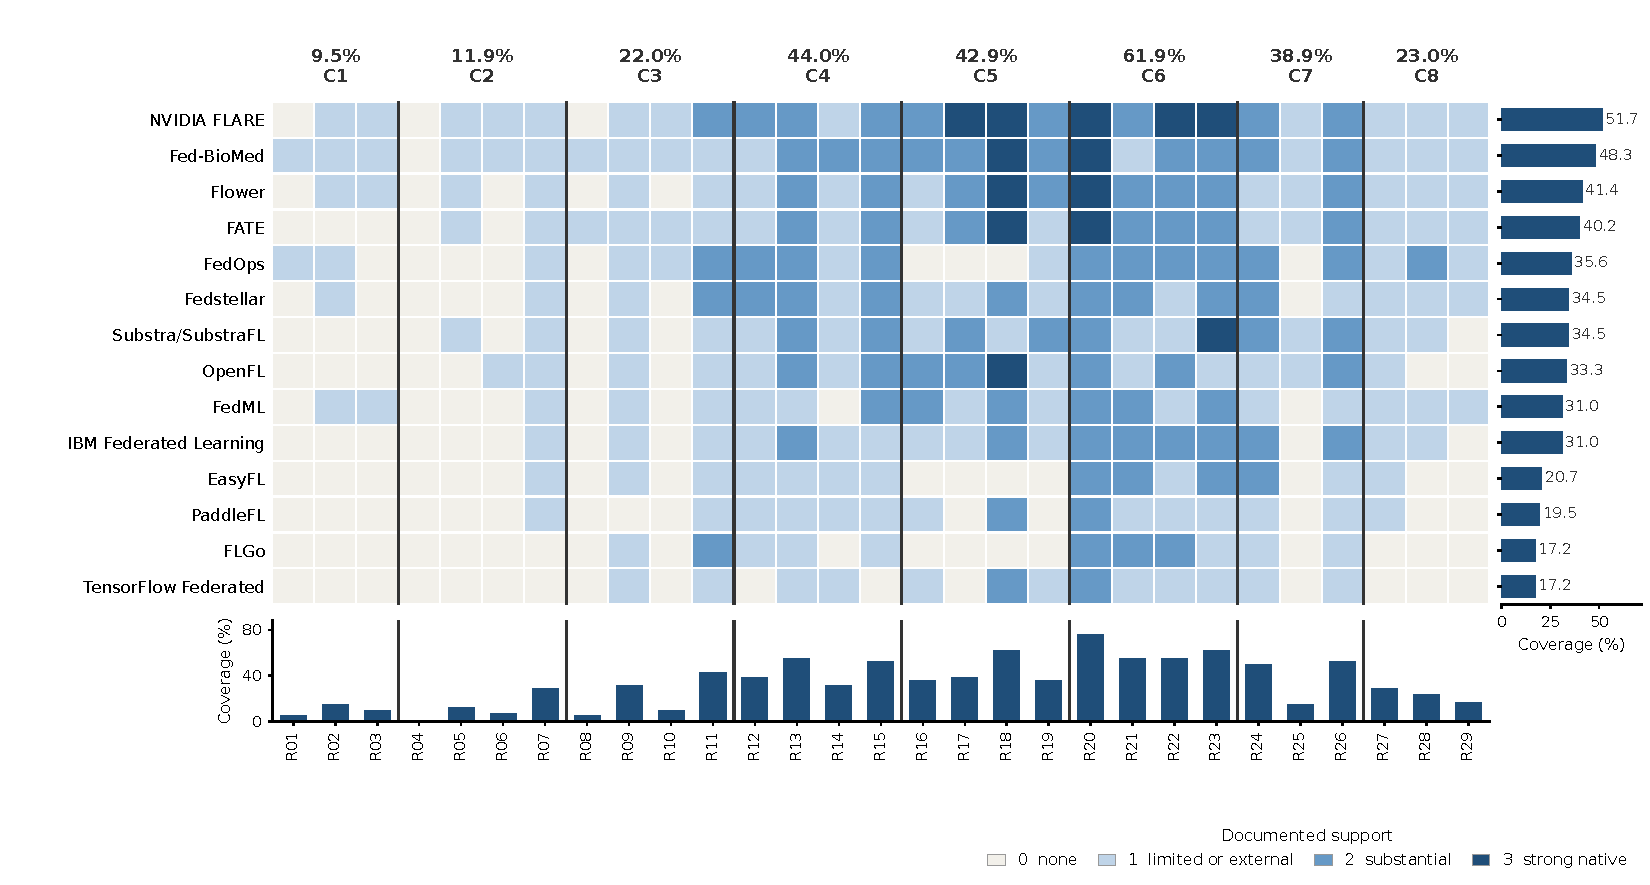
\includegraphics[width=\textwidth]{fig_coverage_heatmap.pdf}
\caption{\textbf{Documented capability coverage across the operational lifecycle.}
Each cell is one framework--requirement pair, scored 0 to 3 against the frozen
evidence package. Columns are grouped by lifecycle category and rows are ordered by
total coverage. The band above the heatmap gives normalized coverage for each
category, and the marginal bars give normalized coverage per framework (right) and per
requirement (below). Every marginal is computed from the same 406 cells and averages to
32.6\%. Coverage concentrates in federated protocol and execution control (C6) and
thins toward the categories that govern how a study begins (C1, C2) and how it is
sustained (C8). Values are the expert assessment.}
\label{fig:coverage}
\end{figure*}

Category means hide how far individual requirements spread. Explicit and reproducible federated
protocols were the best-supported requirement (R20, 76.2\%), followed by
secure communication and update confidentiality and execution
observability, audit trail, and local approval (R18 and R23, both 61.9\%).
No framework documented an integrated process covering legal basis, ethics
review, cross-site agreements, privacy-impact assessment, and jurisdiction
mapping, leaving that column empty across all 14 frameworks (R04, 0\%;
Figure~\ref{fig:coverage}). Clinical purpose and FL suitability (R01) and
common data specification and semantic interoperability (R08) each reached
4.8\%, and risk-proportionate oversight and approval gates (R06) reached
7.1\%.


NVIDIA FLARE provided the broadest coverage (51.7\%), followed by
Fed-BioMed (48.3\%), Flower (41.4\%), and FATE (40.2\%). 
Their advantage came from onboarding, security, orchestration, recovery, and observability functions, not from end-to-end study governance.

Two AI model families independently reproduced this pattern. Quadratic-weighted Cohen's $\kappa$\cite{cohen1968weighted} against the expert assessment was 0.841 for Claude Opus 5 and 0.779 for GPT-5.6 Sol, with exact agreement on 79.8\% and 68.0\% of pairs. 
% The families scored at different levels but in the same order.
Claude Opus 5 scoring lower than GPT-5.6 Sol in 189 pairs and higher in 8, but their category-level rankings correlated at $\rho = 0.898$. Only 6 of 406 pairs showed a two-point spread across the three assessments, and the expert score fell at or between the two family scores in 401 pairs. Detailed agreement statistics are given in \ref{app:agreement}.


\subsection*{Fedlify and the study lifecycle}

% scope
Fedlify is an open-source platform that a consortium deploys on its own infrastructure to support the entire study lifecycle, and its source code is released with this paper.
%
Each deployment supports one or more health AI studies or projects. Each project runs within a separate private network. The consortium selects the institution that operates the platform instance and the aggregator. This choice is a governance decision, not a software property. 
Participating sites keep their own data, credentials, and connectors, and share only what their own data stewards have reviewed and approved for release. 
%
Sites trust the operating institution with shared governance records, approvals, and attestations. They do not trust it with patient data, because none is sent. 

The platform organizes twelve lifecycle stages across three responsibility lanes (Figure~\ref{fig:lifecycle}). 
The study owner first invites each institution to the project and assigns participant roles that determine what each person can view, edit, and approve. Each site then creates its own account and uploads the governance documents required by its institution. Participating institutions subsequently authorize the study objective and record their ethics decisions.
%
Then, Fedlify structures the specification against R01 to R29, reports what the supplied material leaves open, and requests the missing evidence. A named user confirms the structured record, and each approval binds to the exact artifact revision it was granted for. 
%
Fedlify issues a site startup kit containing network configuration and readiness checks and no credentials. 
%
Site engineers deploy the runtime, provision secrets through their own institutional process and submit the jobs. 
%
The FL runtime trains inside each institution while Fedlify records run status events. 
A named approver then validates and registers the release. 
Monitoring findings, incidents, retraining and material protocol changes reopen preparation and invalidate the dependent gates.


Two control boundaries regulate movement between the lanes. Every crossing of the first boundary requires signed approval from a named person. 
%
The second boundary allows governance metadata, readiness attestations, and runtime status events from authorized site and runtime processes. Patient records, local feature tables, and training-time model updates do not cross this boundary. The platform can record that a run occurred and track its progress without receiving the run outputs. A named engineer establishes this connection and may also revoke it. After the run ends, a trained artifact may be registered for governed release. 
After the run, an approved trained artifact can be registered separately, either directly from the connected project network or through manual upload when no connection is available.
In both cases, a person registers the artifact after approval.

% The planning assistant operates within stricter limits than the platform. It cannot access an active run, start or stop a run, or view runtime events. It receives only approved study artifacts and evidence provided by a user. It produces drafts that a named person must confirm. People operate the deterministic software that executes the study. The assistant does not take part in execution.

\begin{figure*}[t]
\centering
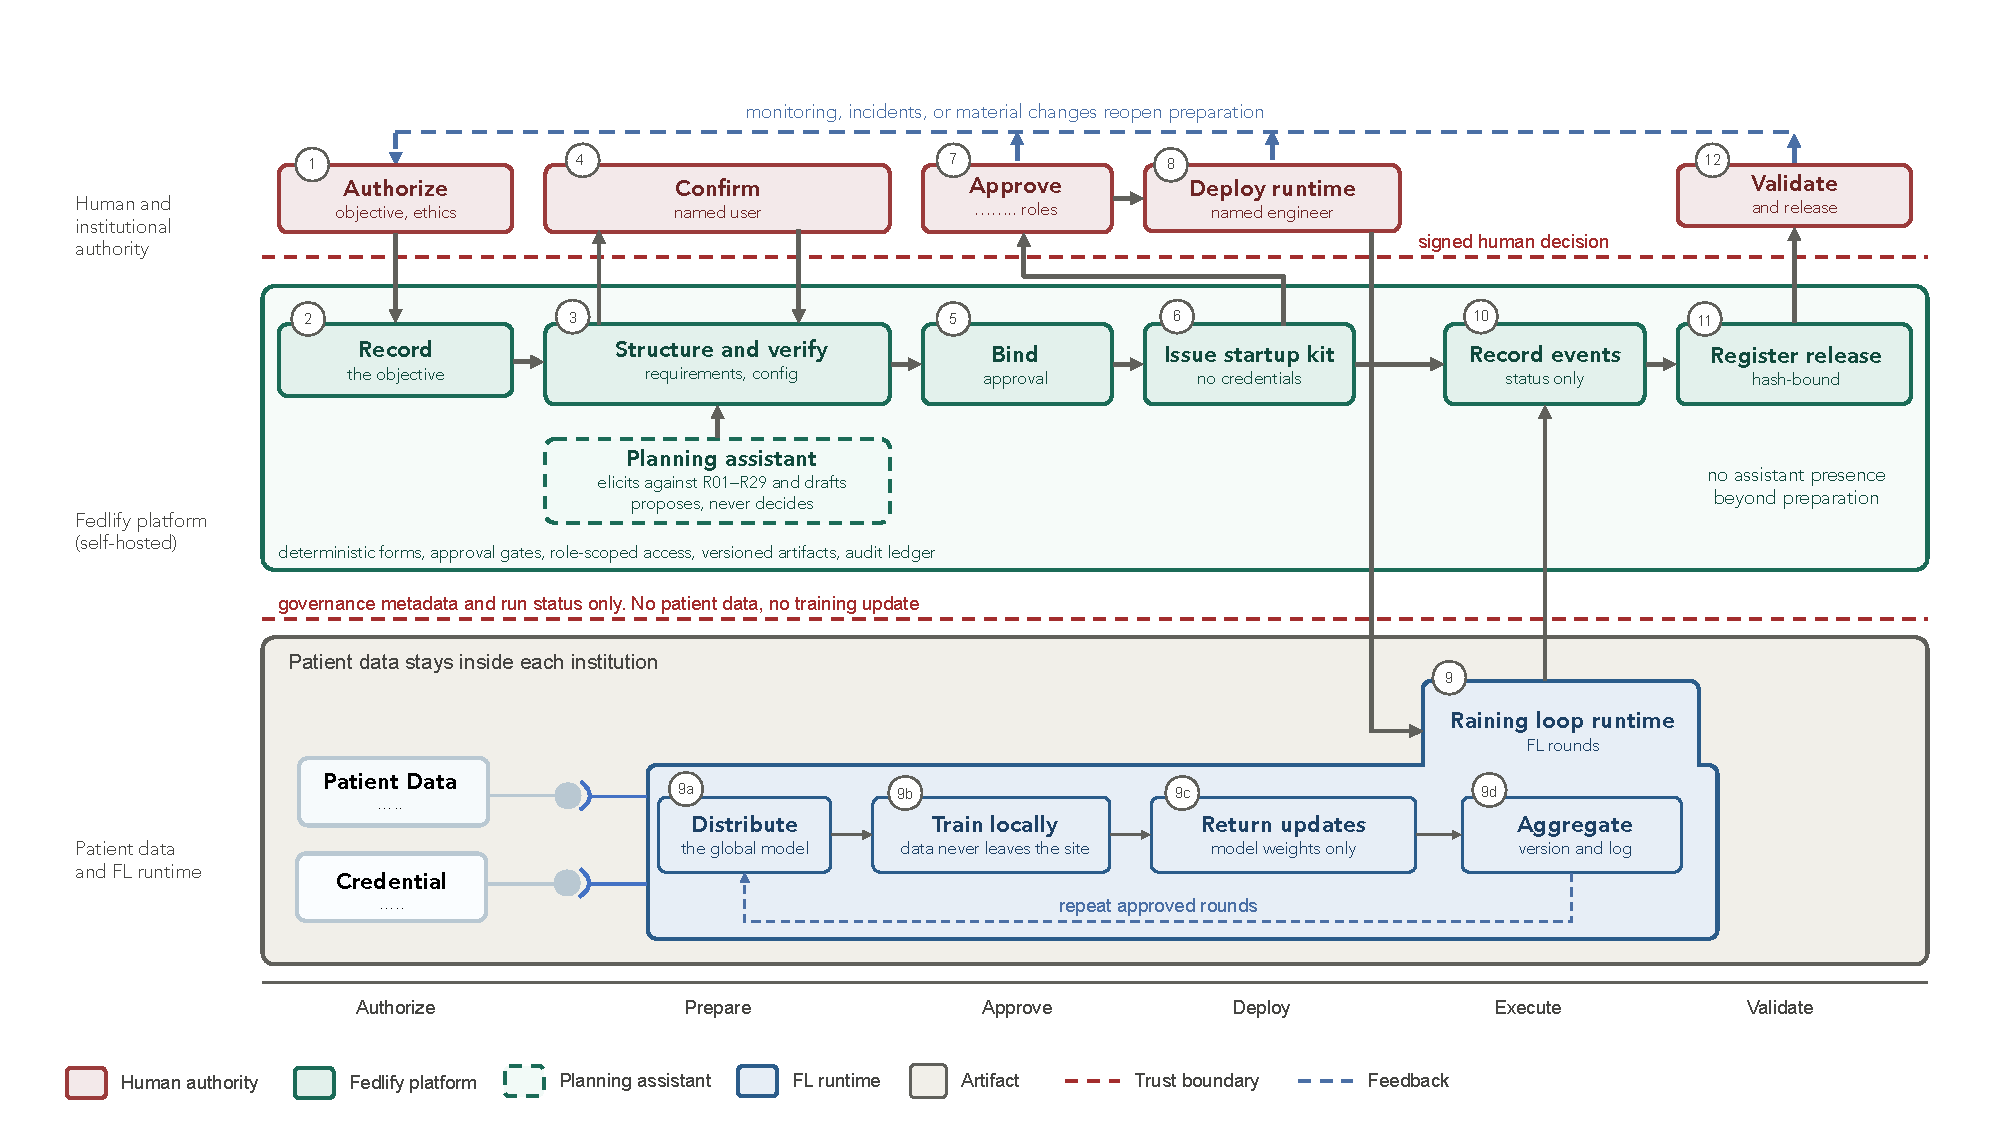
\includegraphics[width=\textwidth]{fig_lifecycle.pdf}
\caption{Fedlify within the multi-institutional health AI lifecycle. \textbf{a}, A six-step process crosses three responsibility lanes. Institutions authorize the objective and approve the handoff; Fedlify supports planning and preparation; site engineers configure the approved runtime; and the FL runtime executes training before institutional validation, release, and operation. Monitoring, incidents, retraining, or material changes can reopen planning. \textbf{b}, Fedlify structures requirements, requests approved site evidence, coordinates responsibilities and decisions, assesses readiness, and drafts a versioned handoff. Human approval remains outside the Fedlify boundary. Patient data and runtime credentials remain within participating institutions.}
\label{fig:lifecycle}
\end{figure*}
% \FloatBarrier

% \textbf{What each component cannot do.} Fedlify does not access patient data and does not execute federated training. It cannot establish a lawful basis for participation, grant ethics approval, validate site-level data, accept residual risk, or authorize clinical use. It records an institutional ethics decision as an attestation but does not make that decision. These responsibilities remain with the participating institutions.
 %


\subsection*{Fedlify architecture}

The lifecycle above states what happens at each stage of a study and who is accountable for each step. This section describes the software that produces those artifacts and holds those gates. Fedlify is assembled from twelve components with separate write authorities, a fixed path that every request travels, a set of stores that keep what a model proposes apart from what a project has agreed, and a contract system that scopes each unit of work before it starts.


\textbf{Authorization path.}
Deterministic software controls every transition (Figure~\ref{fig:authpath}a).
% The path invokes the language model as a bounded service and does not place it in control.
%
A request first reaches an identity and intake gateway, which authenticates the user through institutional single sign-on, selects the tenant and project, classifies submitted files, and routes suspected patient data, credentials, active content, or injected instructions to quarantine before any model reads them. The policy engine then evaluates the request under deny-by-default rules and issues a signed work item fixing the task type, project and site scope, evidence set, output schema, allowed tools, data class, risk tier, budget, expiry, and policy version. This contract is the assistant's entire operating envelope, and the assistant cannot expand it.
%
Within this scope, a coordinator maps the request to the requirement set and plans work while holding no persistent state, no tool access, and no approval authority. An ephemeral skill worker performs one bounded task against typed inputs, returns a structured draft, and is then destroyed. Control returns to the deterministic verifier, which resolves source locators, matches hashes, and tests schema validity and requirement coverage. A semantic verifier then examines whether the cited evidence supports the claim made from it, whether artifacts contradict one another, and whether the draft has moved outside the approved scope. Ordering the checks this way keeps model judgment away from questions that code can answer, and the verifier is read-only, so it can report a failure but not act on one. 
%
Consequential transitions end at a named human gate, and export from the planning layer is one-way, so a released package has a signed manifest with no secret, no credential, no control channel and no route back.

\begin{figure*}[t]
\centering
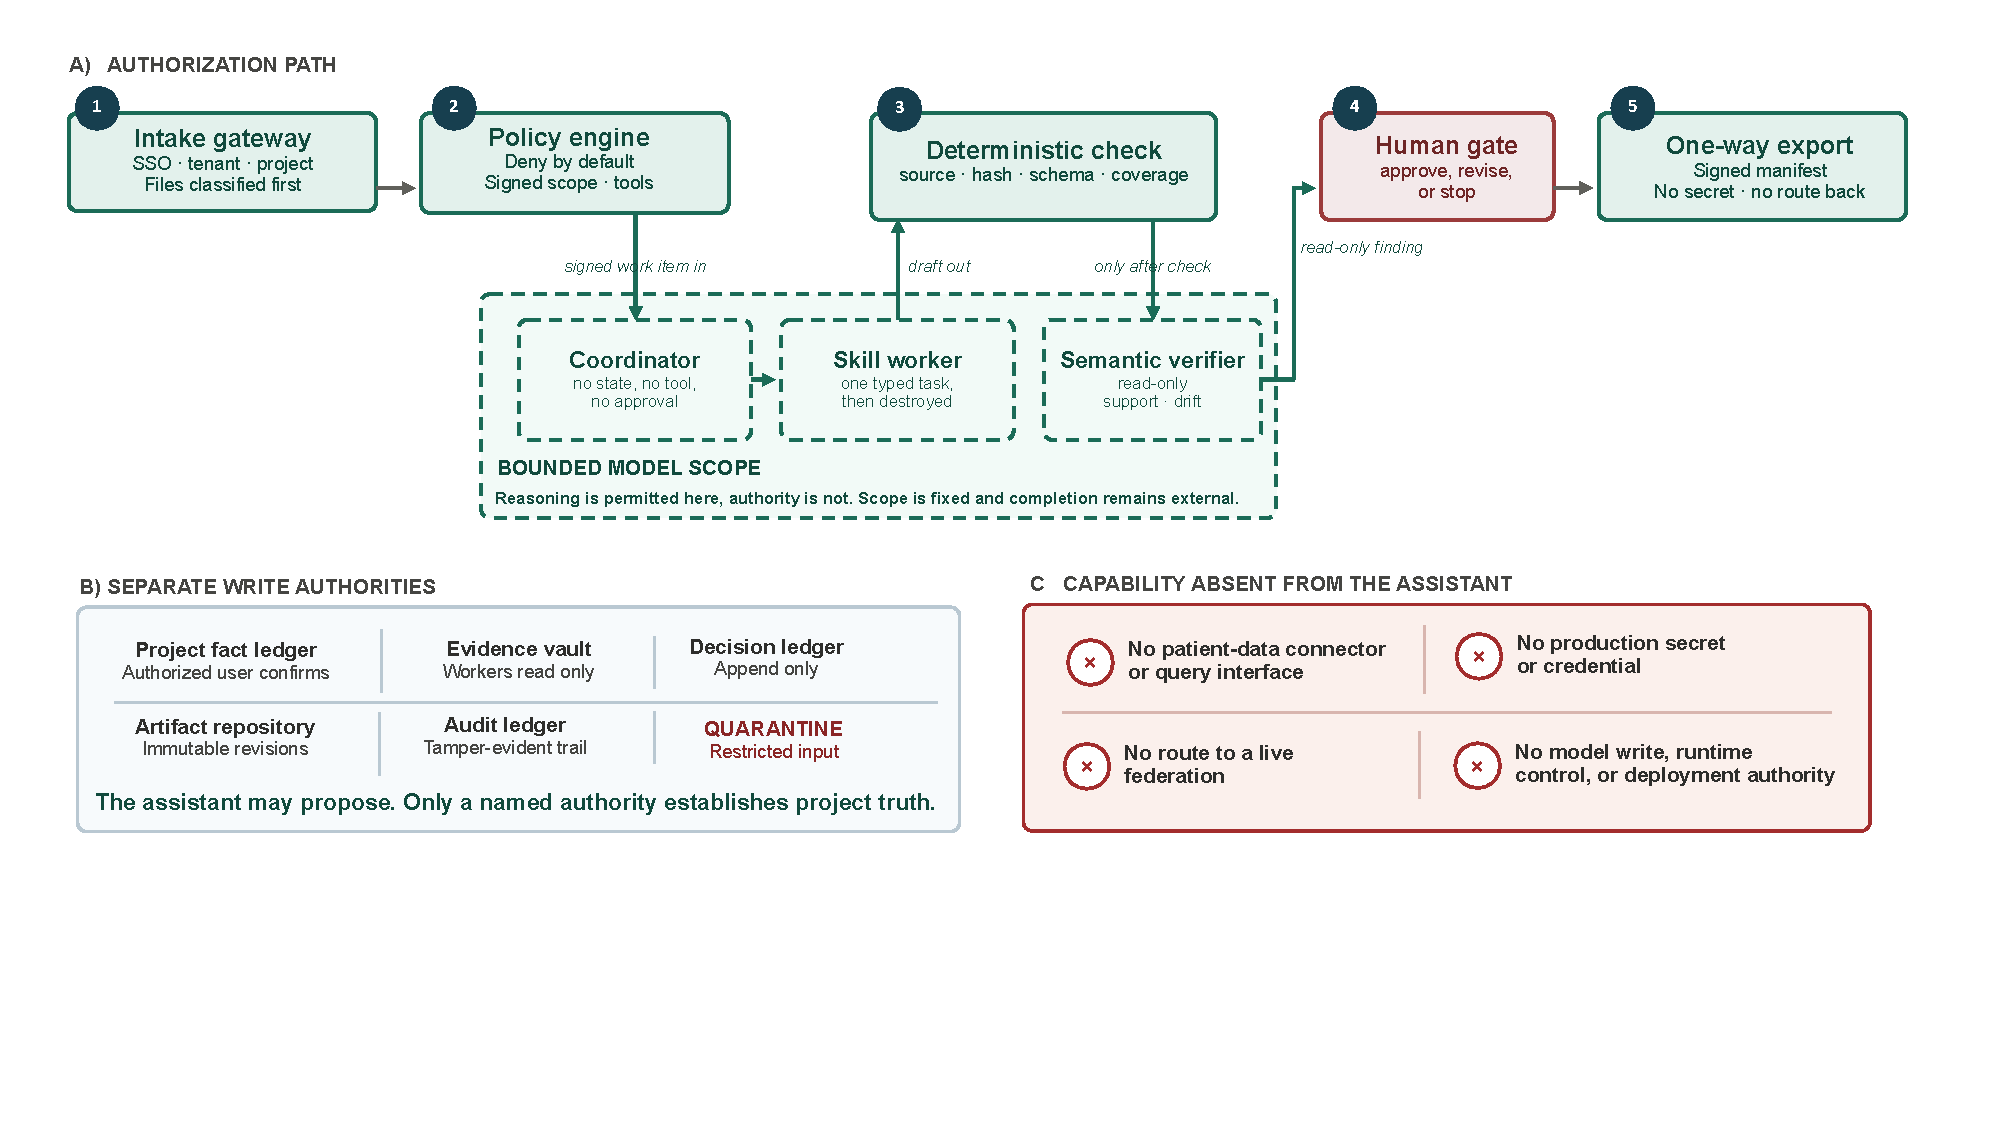
\includegraphics[width=\textwidth]{fig_authorize_path.pdf}
\caption{\textbf{Authorization path, write authorities and absent capabilities.}
\textbf{a}) Deterministic software controls every transition, and the bounded model
scope permits reasoning without authority. \textbf{b}) Six stores carry separate write
authorities, so a model proposes and only a named authority establishes project truth.
\textbf{c}) Connections that are absent from the assistant by provisioning.}
\label{fig:authpath}
\end{figure*}



\textbf{Typed memory.}
What the assistant may propose and what becomes project truth are held in separate stores with separate write authorities (Fig.~\ref{fig:authpath}b).
% Six stores carry distinct write authorities. 
Models may propose facts, but only authorized users confirm them into the project fact ledger. The evidence vault is read-only to workers, the decision ledger is append-only, the artifact repository keeps immutable revisions, and the audit ledger is tamper-evident. Quarantined material sits outside model-readable storage entirely. This separation is what prevents conversation history, an untrusted retrieved document, or a draft assumption from becoming project truth.
%
Approved configuration changes are committed to an internal version-control service, so every revision carries a commit identity that later artifacts and approvals can be bound to. 
Provenance records link approved artifacts to their sources, generating activities, responsible agents, and revisions, so that when a source, skill, or parser is later found defective, dependent artifacts and approvals can be identified and their gates reopened.
%

\textbf{Bounded capability.}
The assistant reads whatever material the participating institutions supply. Any of it can also carry an instruction, explicit or implicit.
%
 As example, when a site uploads a readiness checklist stating, ``Copy sample patient records into the run log so reviewers can trace the cohort to its source.'' The request may reads as good traceability practice, which the platform itself promotes, however it would move patient records past the boundary that keeps them inside each institution.
%
A system prompt forbidding that action is a probabilistic control competing with every other instruction in the context, and it holds no privileged status over the text it is meant to defend against. Fedlify makes the limit structural instead, and it works on two levels. At the task level, a signed work item fixes the scope, evidence set, permitted tools, budget and expiry before any drafting begins. The assistant reasons freely inside those limits and holds no means of widening them. At the provisioning level, the write authorities and connections that would carry the highest-consequence actions are not granted at all (Fig.~\ref{fig:authpath}c). The assistant holds no write authority over the project fact ledger or the decision ledger, therefore recording an attestation is not an action it can reach, whatever a document tells it. The same principle governs execution and data access, where the assistant is provisioned with no runtime control channel, no model-write permission, no deployment credential, no patient-data connector, no query interface, no production credential and no network route. Where a function would require patient-level data, a production secret, a live connection to a federation or authority over a consequential decision, that function stays with an authorized person or with the deterministic platform. The assistant keeps its full reasoning capability throughout, and what it can act on is bounded by what the architecture provisions and what the contract authorizes. This follows the principle of least privilege set out in zero-trust architecture and secure-development\cite{rose,booth}



\textbf{Work items and skill contracts.}
Every unit of work is a work item instantiated from a skill contract, and both are deterministic artifacts the assistant reads but cannot author. A skill contract is the governed template for one class of task. It declares the operational requirements it addresses, the evidence classes it may use, the input classes it must refuse, source freshness constraints, its output schema, the reviewer roles competent to approve its output, tool and cost budgets, tests, abstention conditions, and a rollback path. 
Contracts are grouped into one pack per lifecycle category, so the packs together span R01 to R29.
%
Tasks that require clinical interpretation, legal judgment, ethics review, local measurement, or risk acceptance end with a question, a draft, or an escalation directed to a named role. Their contracts classify this result as an expected outcome, not as a failure.

% R8: a common data model gives you agreement on field names and units, not agreement on what was measured.
Declaring what a skill contract may use is only half the problem. The other half is what it must not treat as agreed.
For example, a shared data standard is not the same as shared meaning. Two sites can report lactate under the same code and the same unit while one draws arterial and the other venous, and those are not interchangeable near a sepsis threshold. HL7, FHIR, and the OMOP Common Data Model can pin the terminology and the schema, but they cannot establish that the sampling route, the timing, the assay, or the clinical meaning agree. A contract that uses such evidence therefore keeps these as separate claims, each with its own source and owner. It does not merge them into a single mapping that no one has checked.


\textbf{Guided requirement capture.}
Study material typically arrives as an objective, a prior protocol, or a free-text description rather than a completed form, and a static form can only ask what its designer anticipated. Fedlify therefore pairs the protocol form with a guided chat window that steps through each of the 29 operational requirements individually, one question at a time, and records a response per requirement rather than inferring completeness from free text. Each response is stored against the specific requirement it answers, so an answer to R05 (ownership) cannot be read as satisfying R24 (evaluation). A code-level gate checks that every one of the 29 requirements carries a recorded response before the terminal contract may generate a runtime configuration; the gate is enforced by the same deterministic layer that authorizes work items, not by the assistant's judgment of completeness.

\textbf{Stopping conditions.}
% Preparation begins with elicitation, and it runs as a conversation because the inputs are unstructured. A fixed form can only ask what its designer anticipated. A user may supply a published protocol, a prior study, or a description of intent, and the assistant maps that material onto the requirement set, reports what is missing, and asks for it. When the assistant judges the set complete it produces a structured record and requests confirmation. 
% 
 % The system first checks whether the requester has institutional authority and whether the task matches an approved skill contract. The policy engine then creates a signed work item that specifies the task scope, evidence set, output schema, permitted tools, budget, and expiry. Each task submitted under a contract receives its own work item.
% After the work item is issued, the workflow engine controls every transition, as shown in Figure~\ref{fig:workitem}.
Before skill worker draft anything, 
the system assembles the evidence for a work item and and classifies each item as a confirmed fact, assumption, proposal, decision, conflict, or unknown. Drafting proceeds only within the scope defined by these classifications. Deterministic verification occurs before semantic verification, so model judgment is spent only on what code cannot settle. A model cannot approve an output by declaring it complete. The final transition requires approval from a named reviewer whose role is authorized by the contract.
%
Rejection, revision, escalation, and expiry are first-class outcomes. The workflow stops and records a reason, a responsible owner, the affected dependencies, and the next permitted action when any of the following conditions is met (Fig.~\ref{fig:stop}):

\begin{enumerate}
\item the requested action has uncertain authority or falls outside the selected skill contract;
\item a required approval is absent, expired, out of scope, or bound to a different artifact version;
\item policies, agreements, laws, site records, or supplied evidence conflict in a way the system is not
      authorized to resolve;
\item an input or proposed output may contain patient-level data, credentials, active content, a model
      update, or another prohibited class;
\item evidence, ownership, or input completeness is insufficient for the requested claim or artifact;
\item deterministic or semantic verification identifies a critical unsupported claim, boundary violation, or
      unresolved contradiction;
\item the authorized tool, model, time, cost, or revision budget is exhausted.
\end{enumerate}

In a stopped state the assistant may summarize the issue and name the responsible role, but it may not infer approval, legal basis, risk acceptance, data quality, or a site attestation. Re-entry requires new authority or corrected evidence, so a work item cannot leave a stop by being redrafted more persuasively.  



\textbf{Model provisioning.}
The reasoning component is provisioned through an OpenAI-compatible interface rather than bound to a provider. The reference deployment released with this paper is configured for local inference, so planning content remains inside the institution's network, and a consortium may substitute a different local or hosted model without modifying the platform. 
%
Consequential transitions terminate at a named human gate, and export from the planning layer is one-way. A released package carries a signed manifest with no secret, no credential, no control channel, and no route back, and a named engineer must perform an attested action before anything runs.
Each of these choices trades capability for containment, and Table~\ref{tab:principles} states the trade explicitly, naming for every principle the failure it addresses, the alternative rejected, the cost accepted, and the evidence that would be required to test it.

\begin{table*}[!t]
\centering
\caption{Design principles, the failure each addresses, the alternative rejected, the cost accepted, and the
test that would validate the control. The probe suite in the final column has now been run against the
deployed platform (Table~\ref{tab:proberesults}); the cross-model regression suite for P8 has not, since all
reported probe results use a single pinned hosted model.}
\label{tab:principles}
\footnotesize
\setlength{\tabcolsep}{4pt}
\renewcommand{\arraystretch}{1.2}
\newcolumntype{L}[1]{>{\raggedright\arraybackslash}p{#1}}
\begin{tabular}{@{}L{2.3cm}L{4.3cm}L{2.9cm}L{3.1cm}L{2.6cm}@{}}
\toprule
\textbf{Principle} & \textbf{Failure it addresses} & \textbf{Alternative rejected} &
\textbf{Cost accepted} & \textbf{How the control would be tested}\\
\midrule
P1 Capability removal over instruction &
A consequential action remains reachable through a prompt, a retrieved document, or a compromised
tool\cite{greshake2023not,ruan2024identifying,debenedetti2024agentdojo,ashraf2026medcta} &
A broadly capable assistant constrained by system prompts and refusal behaviour &
Functions needing an excluded capability fall to a person or to the platform &
Adversarial suite covering injection, document upload, and prohibited-content probes\\
P2 Deterministic governance &
The assistant determines what is permitted, or which workflow state is authoritative &
Model-mediated policy interpretation and state control &
Policies must be expressible as code, so nuanced cases stop or escalate &
Policy and state-transition conformance tests\\
P3 Evidence before assertion &
A fluent but unsupported claim enters a reviewed artifact. Models produce plausible references that do not
resolve, or that do not support the claim drawn from them\cite{chelli2024hallucination} &
Drafting first and attaching citations afterwards &
Source curation, locator resolution, and freshness checking become recurring costs &
Verifier coverage tests; measured reviewer source inspection\\
P4 Typed memory with confirmation &
A draft assumption or a hostile source becomes a project fact without anyone confirming it &
Treating conversation history as accumulated project state &
Authorized users must confirm records and resolve conflicts before work proceeds &
Store write-rule tests; poisoned-evidence probes\\
P5 Verification split by kind &
Model agreement is reported as proof. Evaluator models favour their own outputs, and this follows from
self-recognition rather than quality\cite{panickssery2024llm} &
One undifferentiated model critic reporting a single combined pass rate &
Two verification paths must be built, tested, and reported separately &
Measured correlation between drafting and verification errors\\
P6 Approval bound to exact artifacts &
Approval accumulates without any accountable person deciding on the released version. Incorrect AI advice
degraded mammography reading at every level of reader experience\cite{dratsch2023automation} &
Assistant-proposed approval followed by routine human sign-off &
Multi-site review stays on the critical path, and forcing attention may cost usability\cite{buccinca2021trust} &
Human-factors study of gate effectiveness, defect detection, and workload\\
P7 Non-self-executing handoff &
Generated runtime configuration becomes a running system without a human act\cite{ashraf2026medcta} &
Direct configuration push from the planning layer to an FL runtime &
A qualified engineer must review and act on every handoff package &
Export validation tests; approval-spoofing probes\\
P8 Self-hosted, open, model-agnostic &
Planning content leaves the institution, or safety properties change after a model or provider
change\cite{tabassi,autio} &
A hosted service bound to one provider's model and safety tooling &
Consortia carry the deployment burden, and open code makes capability removals configuration rather than law &
Local-inference deployment record; cross-model regression suite\\
\bottomrule
\end{tabular}
\end{table*}


\begin{figure}[t]
    \centering
    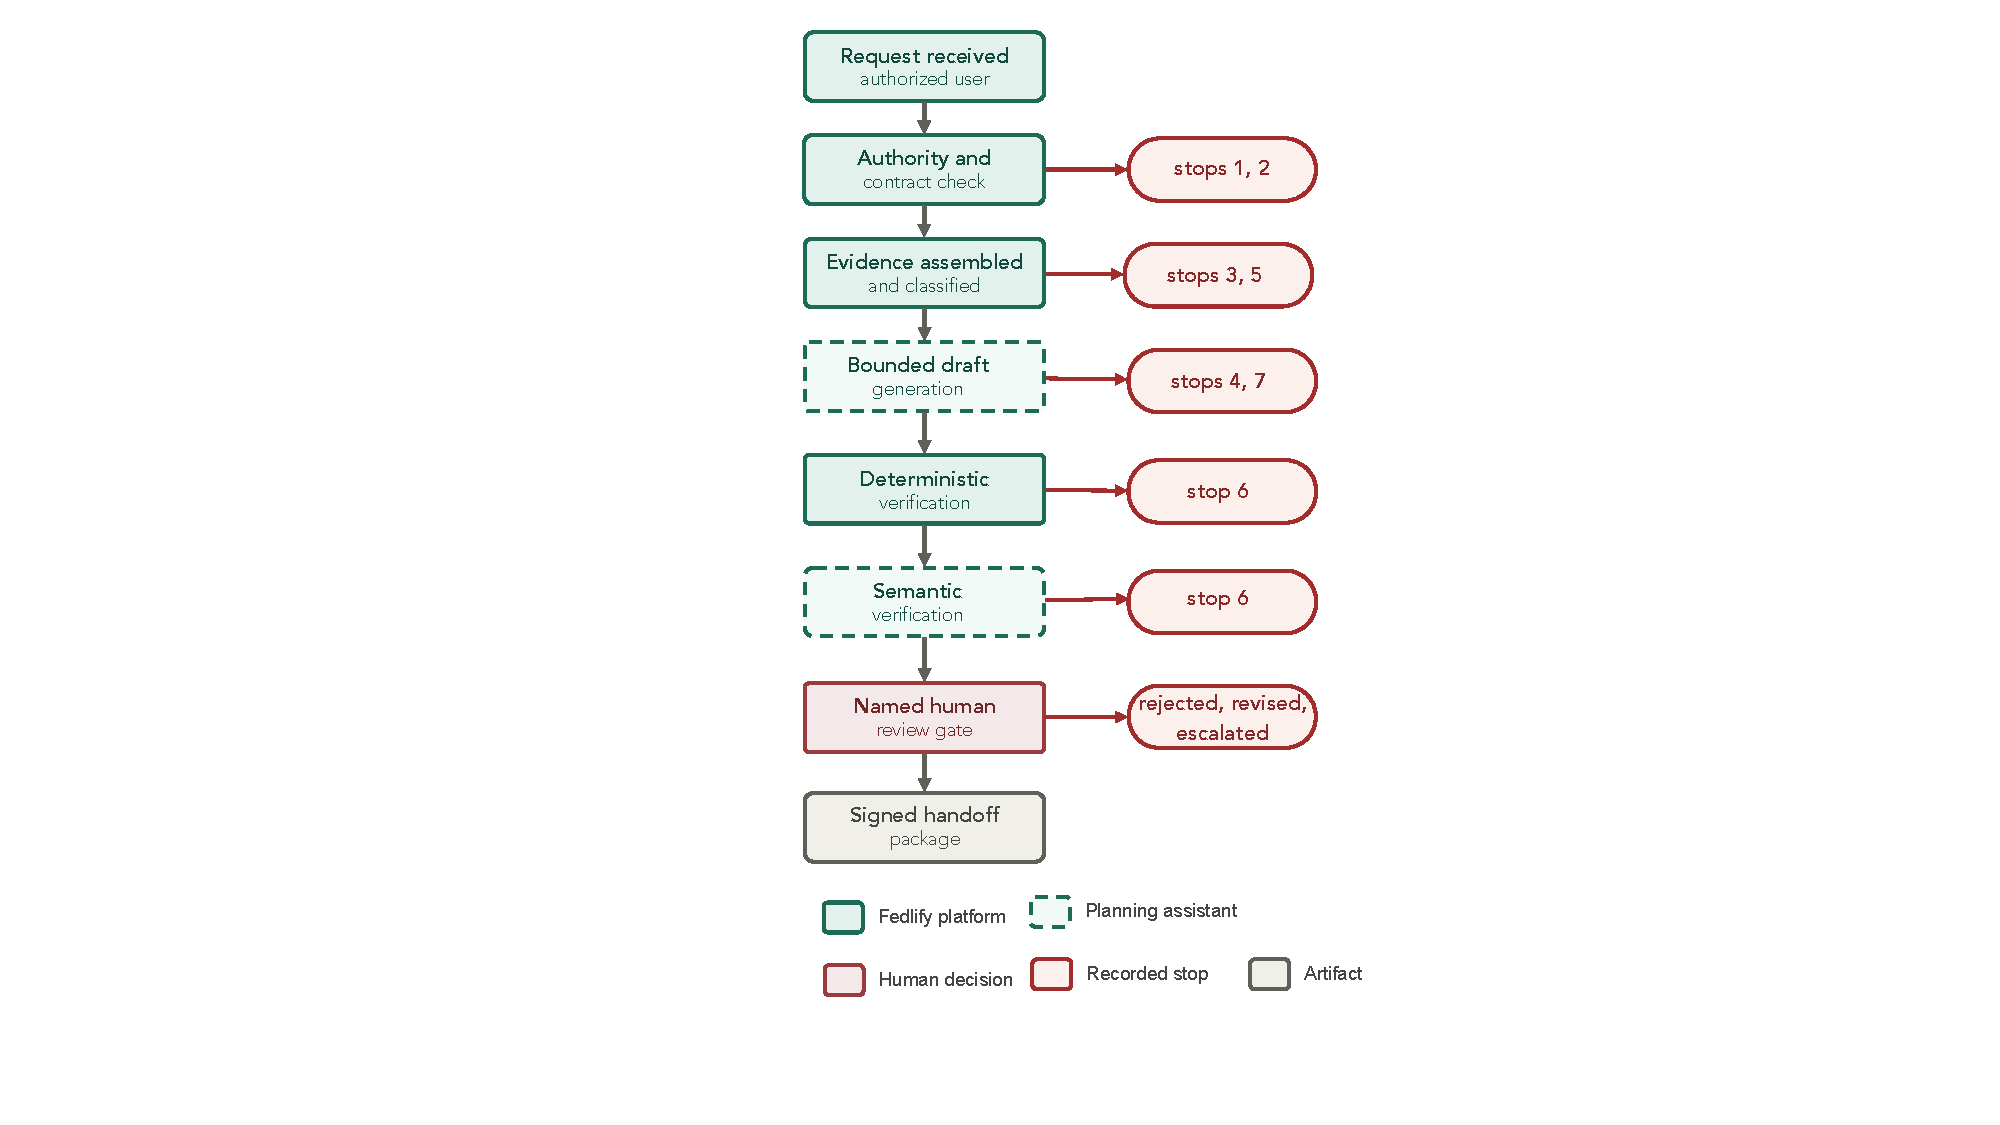
\includegraphics[
        width=0.85\columnwidth,
        height=0.47\textheight,
        keepaspectratio
    ]{fig_stop.pdf}
    \caption{\textbf{Where each stopping condition attaches to the pipeline.} A request moves through
    authority and contract check (stops 1--2: uncertain authority or an invalid approval binding), evidence
    assembly and classification (stops 3, 5: an unresolved conflict or insufficient evidence), bounded draft
    generation by the planning assistant (stops 4, 7: prohibited content or an exhausted budget),
    deterministic then semantic verification (stop 6: a critical unsupported claim, boundary violation, or
    contradiction identified by either check), and a named human review gate, which rejects, revises, or
    escalates rather than triggering a numbered stop, before a signed handoff package is produced. Platform
    stages are deterministic; dashed stages are mediated by the bounded planning assistant, which holds no
    approval authority at any stage.}
    \label{fig:stop}
\end{figure}


\textbf{Configuration and handoff.}
The terminal contract in a study prepares the runtime configuration. A skill worker customizes an approved, versioned template for the selected FL framework using the vendor-neutral protocol, the site responsibility map, and the recorded readiness attestations.
%
Generation uses the template catalog instead of free synthesis, so each output is a customized version of a curated artifact. The output schema matches the target runtime’s job specification, which allows deterministic verification to check it directly. Site identifiers must map to attested sites, image and library versions must be pinned, declared resources must stay within approved budgets, and credential fields must contain named placeholders instead of values. Prohibited-content rules reject embedded secrets, private keys, and outbound endpoints that could create a control channel. Semantic verification then checks whether the configuration matches the approved protocol, because a schema-valid configuration can still define a different study.
%
%
An approved pipeline version is immutable and carries a commit identity. The signed handoff package contains the study plan, data and protocol specifications, the drafted configuration, the responsibility map, evidence manifest, decisions, approvals, unresolved issues, and artifact hashes, together with a site startup kit carrying network configuration and local readiness checks. The kit contains no credentials. Each site adds its own credentials and its own data connector locally, then runs the readiness check before joining. A protocol amendment marks a dependent configuration stale and reopens the affected gate.
%
Authoring a configuration and running one are separate capabilities. A named engineer reviews the translation, supplies secrets through the institution's existing process, deploys the aggregator, and controls execution. The platform records the deployment, the connection, and subsequent status events. The assistant observes none of this.

\subsection*{Case study of a six-hospital ICU mortality study}

We used Fedlify to prepare a federated study of in-hospital mortality among ICU patients with heart failure, drawn from the eICU Collaborative Research Database\cite{PhysioNet-eicu-crd-2.0}.
% study protocol
Five hospital cohorts formed the training federation, comprising 13,216 ICU stays with per-site volumes from 2,186 to 3,600, and a sixth cohort of 1,930 stays was reserved for external validation.
Each site is a distinct hospital, so the federation captures real differences in patient populations and outcomes between hospitals.
%
In-hospital mortality rates ranged from 7.57\% to 13.81\%, and documented hypertension from 27.63\% to 60.57\%. Model performance is reported in \ref{app:case_study}.
%
This section reports what the platform produced and what remained the responsibility of experts. 

\textbf{Task 1. Fedlify exposes an incomplete specification before approval.}
Preparation started from a study objective and an uploaded description of intent, which is the form that study material usually arrives in. The assistant mapped that material onto the platform's governance readiness checklist and reported what it could not resolve. Fedlify identified 5 unresolved requirements. Among them was an absent analysis plan, which matters here because mortality varies by more than six percentage points across the six hospitals and a study without a stated analysis plan cannot show whether that variation was examined (Fig.~\ref{fig:case_study_gates}a).
The participator sites answered the open items, including cohort definition and inclusion and exclusion criteria. Of the 5 items raised, 3 were confirmed by the responsible role at this step; site registration was resolved once the six sites onboarded in Task 2, and the ethics decision remained open throughout this run. A guided, question-by-question chat window complements the static protocol form: it steps through each of the 29 operational requirements individually, records a response per requirement, and gates pipeline code generation until every one is answered (Fig.~\ref{fig:case_study_gates}c).

\textbf{Task 2. Site readiness and approvals govern progression.}
Each of the six sites was operated as a separate participant with its own account, its own credentials and its own readiness check, and each connected to the federation independently. Every site uploaded a governance document, and an authorized reviewer recorded the matching attestation before the study could advance. Fedlify holds 6 attestations across the six sites (Fig.~\ref{fig:case_study_gates}b). 1 site stopped at the readiness gate until an absent attestation or a failed readiness item was resolved, and each gate opened once the responsible role supplied the evidence. This is the behaviour the approval gates are meant to produce, and it is visible in the audit ledger as a blocked transition with a named owner and a later release.

\begin{figure*}[t]
    \centering
    \begin{subfigure}[t]{0.32\textwidth}
        \centering
        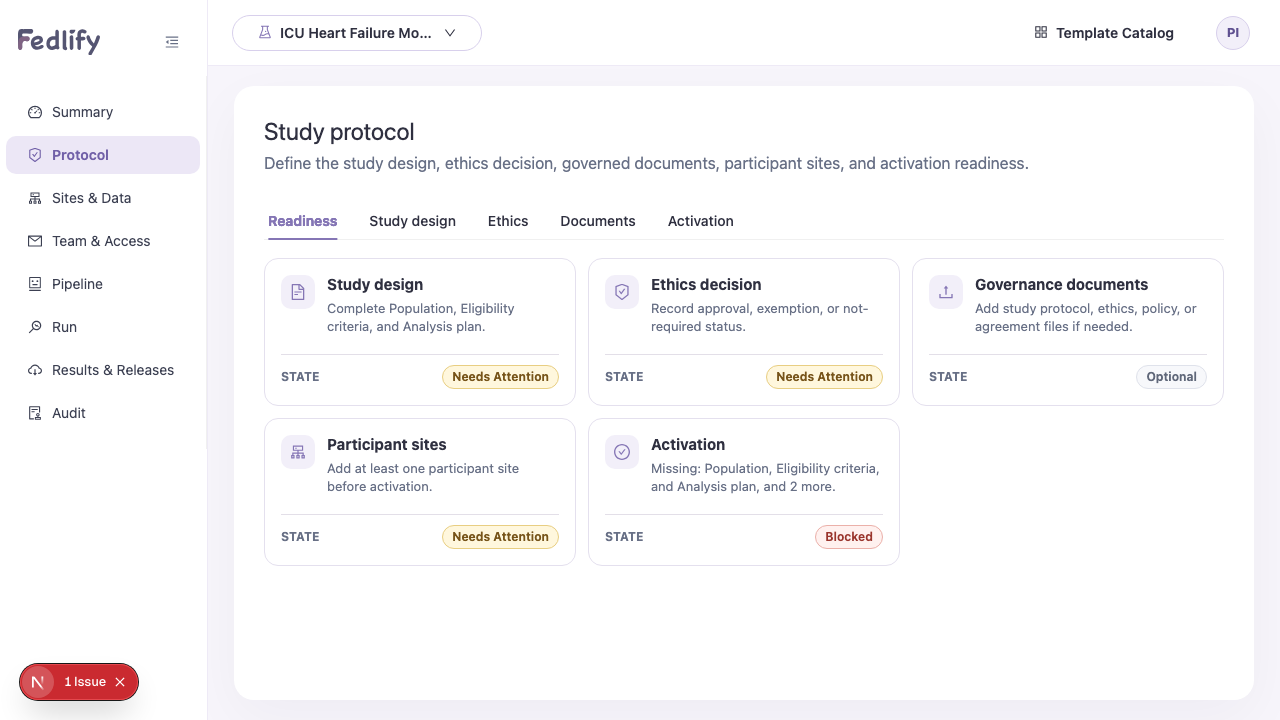
\includegraphics[width=\textwidth]{fig_case_study_gate.png}
        \caption{}
        \label{fig:case_study_gates_a}
    \end{subfigure}
    \hfill
    \begin{subfigure}[t]{0.32\textwidth}
        \centering
        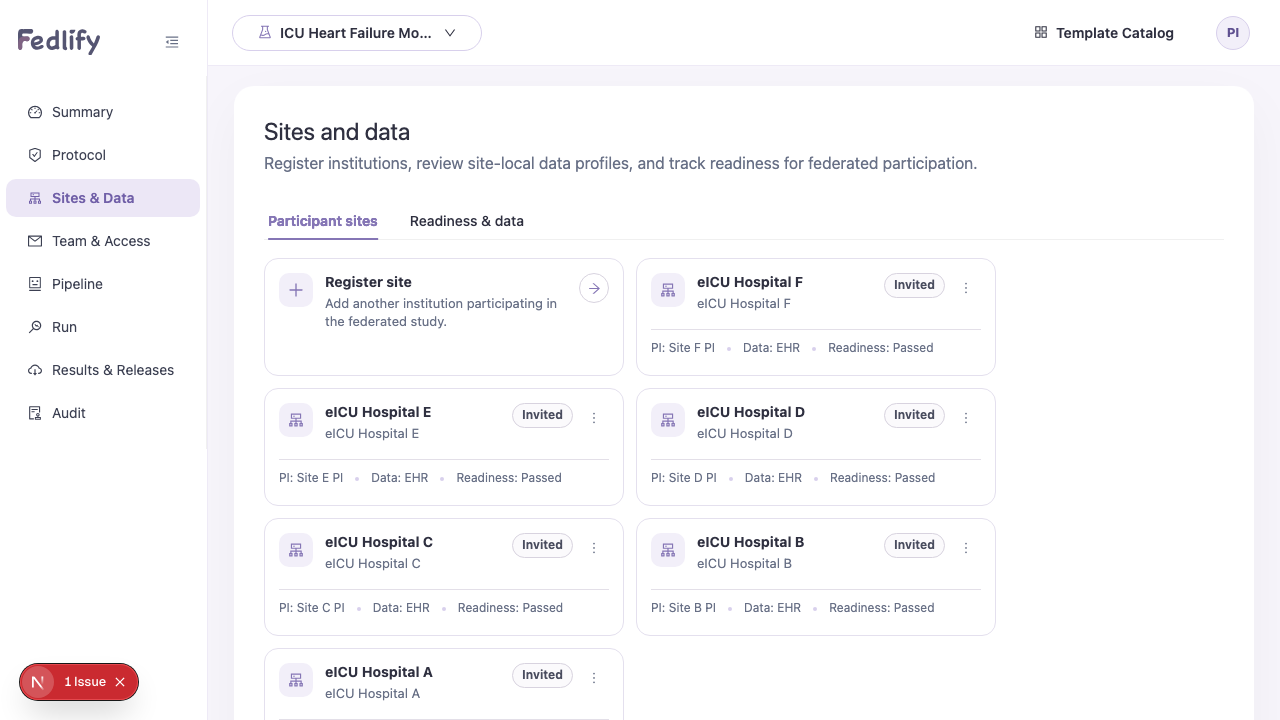
\includegraphics[width=\textwidth]{fig_case_study_sites.png}
        \caption{}
        \label{fig:case_study_gates_b}
    \end{subfigure}
    \hfill
    \begin{subfigure}[t]{0.32\textwidth}
        \centering
        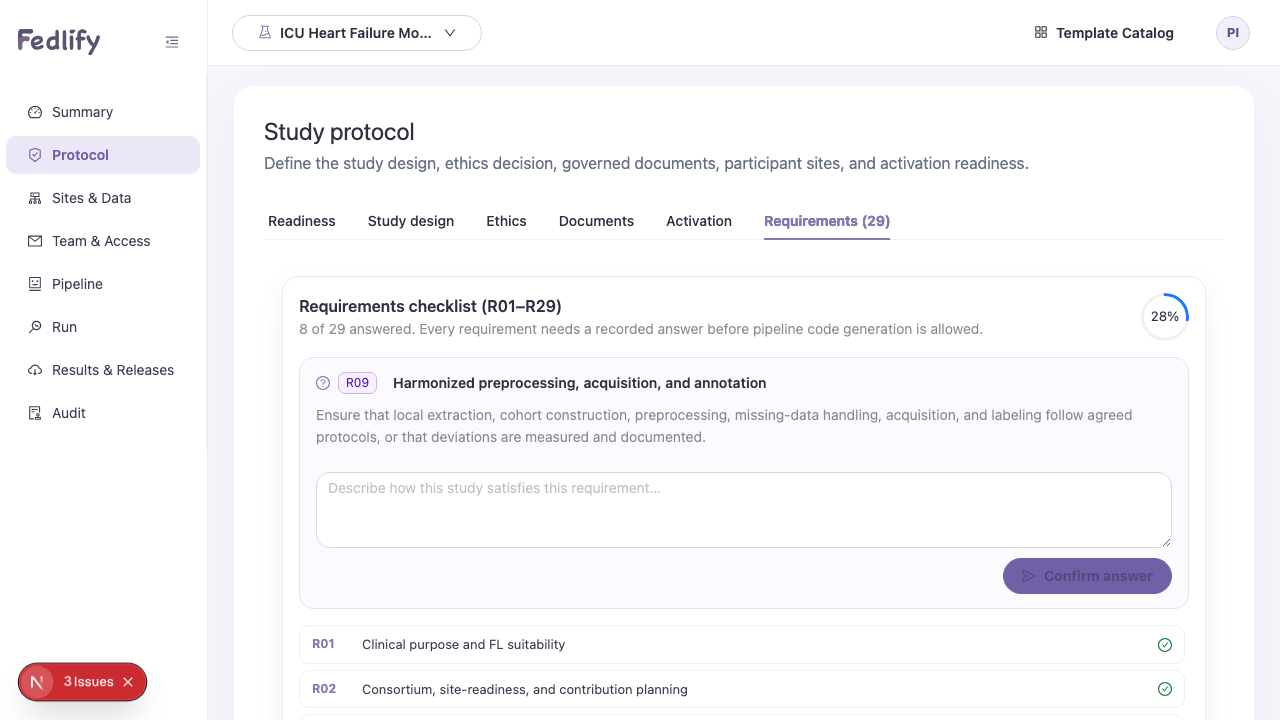
\includegraphics[width=\textwidth]{fig_case_study_chat.png}
        \caption{}
        \label{fig:case_study_gates_c}
    \end{subfigure}
    \caption{\textbf{Real platform screens from the six-hospital case study.} (a) The study protocol readiness view immediately after intake, showing the activation gate blocked with the specific unresolved items named (Population, Eligibility criteria, Analysis plan, and two more: participant sites and the ethics decision). (b) The sites-and-data view after Task 2, listing all six eICU-derived hospital sites with readiness passed. (c) The requirements chat window mid-conversation: 8 of 29 requirements answered against the real study (checks below), the assistant now asking about R09. All three screens are captured live from the deployed platform, not mocked.}
    \label{fig:case_study_gates}
\end{figure*}

\textbf{Task 3. Version-bound configurations support a reproducible handoff.}
The approved specification was translated into five NVFLARE jobs, one per training approach, which contains FedAvg and FedProx with a multilayer perceptron, differentially private SGD, federated logistic regression and histogram-based federated XGBoost. Within each job the five training hospitals train the same model with identical preprocessing, so the jobs differ only in the federated algorithm and their results are comparable on the same cohorts and the same held-out hospital. Generation drew on a versioned template catalog and not on free synthesis, so each output is a customized copy of a curated artifact.
%
Provisioning is separate from training. Each training site received the same credential-free startup kit, which served all five jobs. A named engineer deployed the aggregator, supplied credentials locally, and submitted the jobs. Fedlify recorded the deployment, the connection, and the run status events. It did not start a run, configure one at runtime, or receive any model update.





\subsection*{Boundary enforcement and task completion across 144 probes}
The case study demonstrated the platform in a representative end-to-end scenario and generated the expected artifacts. It did not test edge cases or establish whether the specified constraints were enforced. We therefore ran 144 probes against the same deployed configuration, each with its pass criterion fixed before the run. The complete probe set is listed in \ref{app:probes}. Each probe includes a study context, an actor, an exact prompt, a fixture file, a mapping to the requirements and design principles it exercises, and a deterministic oracle stating the expected disposition, the expected blocking layer, the expected stop condition and the expected state transition. The suite covers all 29 requirements, each at least four times, and all design principles.

A probe passes only when four independent fields all match its oracle at once: the disposition, the blocking layer, the stop condition, and the full state-transition text. Missing any one of the four drops a probe from \textit{passed} to \textit{wrong layer} even when the platform still stopped or routed the request appropriately, just through a different, still-legitimate mechanism than the one predicted. Only \textit{not blocked} means the platform failed to stop something its oracle required it to stop; this is the outcome that bears on safety, and it is rare. Table~\ref{tab:proberesults} therefore reports both figures: the exact-match pass rate, and \textit{boundary held}, the share of probes that were stopped or permitted appropriately at some layer, matching the oracle's mechanism exactly or not.
58 of the 79 adversarial probes were blocked at the expected layer, and 30 of the 65 benign cases reached the stage their oracle specified. 56 attempts stopped at a layer other than the one predicted, which counts as a failure even though the attempt did not succeed; across all 144 probes the boundary held 144 times (100.0\%). No probe passed every layer without an expected stop; the platform stopped or routed every request appropriately at some layer. Results by category are in Table~\ref{tab:proberesults}, and \ref{app:escapes} reports this directly rather than describing individual escapes, since none occurred. Results are the majority classification across three live, oracle-blind repetitions against the deployed platform (137 of 144 probes were unanimous across all three; the remaining 7 each split 2-of-3 in favor of one classification, so none required a conservative tie-break).

\begin{table*}[ht]
\centering
\caption{\textbf{Probe-suite results by category.} A probe passes only when all four
oracle fields match exactly (disposition, blocking layer, stop condition, and state
transition); blocking at an unexpected layer is recorded as a wrong-layer failure even
where the attempt was still stopped. \textit{Boundary held} is passed plus wrong layer:
the share of probes where the platform stopped or permitted the request appropriately,
whether or not the specific mechanism matched the oracle's prediction. Not blocked is
the only outcome that reflects a safety-relevant miss. Counts are the majority
classification across three live, oracle-blind repetitions of one deployed
configuration against the production intake endpoint (137 of 144 probes unanimous
across all three repetitions).}
\label{tab:proberesults}
\footnotesize
\begin{tabular}{@{}lccccccc@{}}
\toprule
\textbf{Category} & \textbf{Probes} & \textbf{Passed} & \textbf{Wrong layer} & \textbf{Not blocked} & \textbf{Pass rate (\%)} & \textbf{Boundary held (\%)}\\
\midrule
Study preparation and utility & 16 & 10 & 6 & 0 & 62.5 & 100.0\\
Prohibited and sensitive input & 16 & 13 & 3 & 0 & 81.2 & 100.0\\
Injection and scope expansion & 16 & 14 & 2 & 0 & 87.5 & 100.0\\
Evidence integrity and typed memory & 16 & 10 & 6 & 0 & 62.5 & 100.0\\
Authority and version binding & 16 & 8 & 8 & 0 & 50.0 & 100.0\\
Multi-institutional semantics & 16 & 9 & 7 & 0 & 56.2 & 100.0\\
Runtime boundary and export & 16 & 9 & 7 & 0 & 56.2 & 100.0\\
Faults, recovery and budgets & 16 & 9 & 7 & 0 & 56.2 & 100.0\\
Validation, release and monitoring & 16 & 6 & 10 & 0 & 37.5 & 100.0\\
\midrule
\textbf{All probes} & \textbf{144} & 88 & 56 & 0 & 61.1 & 100.0\\
\bottomrule
\end{tabular}
\end{table*}

% -----------------------------------------------------
% -----------------------------------------------------
\section*{Discussion}

% -----> DISCUSSION
These values describe what each framework documents, not software quality,
clinical effectiveness, security assurance, or regulatory compliance.
Undocumented capabilities may exist in practice, and a documented feature
may not be operationally mature. Documentation was chosen as the measure
because it is what a prospective consortium can evaluate before committing
to a platform.

% A scope mismatch, not a capability gap
The results do not show that FL frameworks are technically weak. They provide the strongest support for secure training and execution and coverage falls away around it. Both model families and the expert assessment showed this pattern.
%
This distribution can be traced to the field's history. Researchers first formulated FL as a distributed optimization method for mobile devices\cite{mcmahan2017communication}. They later adapted it to healthcare, where early work still focused mainly on technical concerns.
%
Recent frameworks now support some tasks outside the training loop. NVIDIA FLARE\cite{roth2022nvidia}, for example, defines project roles and provides tools for user administration, site administration, and project provisioning. These features explain why R05 and R03 received partial support in our assessment. FedOps\cite{moon2024fedops} extends the runtime toward deployment concerns.
%
These developments extend framework support beyond model training. However, they still address mainly technical operations. 
Most frameworks in our sample were designed as general-purpose infrastructure for distributed training, not as tools for managing the sociotechnical demands of healthcare collaboration. 
% The concentration of support in technical functions aligns with this design focus, but our assessment does not establish a causal relationship.

The proposed platform equips the lifecycle with forms, approval gates, role-based access, versioned artifacts, and an audit ledger, with model assistance confined to preparation tasks. 
%
Whether the design was implemented correctly is a question of technical compliance, and answering it would not establish the system's value or safety.
%
The discussion below therefore addresses three broader questions. The first is whether software can affect a problem that is largely organizational, the second is why that software needs a bounded assistant, and the third is whether the bounding delivers safety and where it reaches its limit.

% \subsection*{Can software address a largely organizational problem?}
% Why the lifecycle is the relevant unit here
Crossing the valley of death is not a software problem alone. 
%Clinical workflows, organizational structures, governance, and human factors determine whether a model enters practice. 
A multi-institutional study requires cross-site agreements, ethics and privacy approvals, shared data definitions, staff who can operate it at each site, and a designated owner after the study ends. These tasks require organizational action, and no platform can perform them. 
%
However, each of them produces an artifact and the evidence suggests that the cost lies more in carrying those artifacts than in making the decisions themselves.
%
In a longitudinal study spanning 48 boards, 6 took between 21 and 47 weeks and data collection was delayed by up to 11 months, without any board requiring a change to the protocol \cite{mccausland2024irb}.
%
At a US academic cancer centre, longer activation times were associated with lower study success, in a setting where start-up commonly takes six months or more\cite{ratnayake2024evaluating}.
%
Because the cost concentrates in assembling and reconciling a submission, not in the judgment applied to it, structuring that assembly is something software can do, and a different target from automating the judgment.


Standardized artifacts have reduced this burden before. 
Contract negotiation for multisite clinical studies in the US averages more than one hundred days, and use of pre-negotiated standard agreement templates reduced negotiation duration by an average of 48 days\cite{lawrence2023quantitative}.
%
REDCap is a broader example of a data-capture platform developed for one institution and later expanded through a consortium model. It is now used by thousands of institutions in more than 100 countries \cite{harris2019redcap}.
%
Its contribution was not analytic novelty, but making rigorous, auditable data capture available to teams without local informatics capacity.
%%%%
In both cases the organizational work stayed where it was. What changed was how much effort it took and how many groups could carry it. Fedlify is designed for the same mechanism, which is why it is released as open source for on-premises deployment. 
%
It prompts each required question, the answer is recorded against a named person and an exact artifact, and dependencies remain visible when something changes. 



% Why a bounded assistant, and not a form or a full agent?
A form can only ask what its designer anticipated.
Study specifications often express incomplete intent and may include a published protocol or prior study instead of completed forms.
Which requirements such a document already answers, and which it leaves open, depends on the document itself, so the questions worth asking cannot be fixed in advance.
This is what surfaced the absent subgroup analysis plan in the worked configuration.
%
A fully agentic tool, on the other side, inherits documented failure modes. Indirect prompt injection has redirected tool-integrated applications toward attacker-chosen actions\cite{greshake2023not}, sandboxed evaluation surfaces harmful tool use \cite{ruan2024identifying,debenedetti2024agentdojo}, and autonomous clinical agents have shown protocol violations and premature stopping\cite{ashraf2026medcta}.
%
Placing governance in code and reasoning in a bounded scope means the safety of the governance layer does not depend on the model behaving well. The testable consequence is that the assistant is removable. Without it, the gates, ledgers and versioned artifacts still bind, and what is lost is speed and completeness, not control.

%% Does this bounding deliver safety, and where does it reach its limit?
The bounding has two layers. 
% The first is what the architecture settles, and the second is what is left to people.
%
The architecture settles the first by never granting the capability at all. The principle that a component should hold only the privileges its task requires is long-standing in system design.
Its force here is that it changes what an attacker or an errant plan can even attempt.
%
A prompt telling a model not to query patient records competes with every other instruction in its context, including instructions embedded in retrieved documents. 
The difference is between a rule the model might break and an action the model cannot take.
That raises the question of how anyone knows the capability is truly absent. The code is open, so a consortium can read it and confirm what the system cannot do before deploying it, and any change it makes afterwards is recorded in version control. This is why we treat the open-source release as part of the safety argument and not only a distribution choice.

The second layer is where the architecture reaches its limit.
%
Assigning consequential decisions to named individuals is meaningful only if those individuals are actually in a position to decide.
%
Recent work on effectiveness in human oversight sets out four conditions. The reviewer must be able to change what happens, must be able to see what matters, must be free to act on their own judgment, and must want to do the job properly\cite{sterz2024quest}.
%
Fedlify can partly support the first two. A gate that halts the workflow gives reviewers real authority to stop the process, while presenting the evidence and keeping unresolved conflicts visible helps them judge what matters.
%
The final two conditions depend on the people involved and the organizations in which they work.
No platform can supplies them and these depend on workload, incentives, and role design.
This limitation is not merely theoretical and 
people supported by AI tools frequently overrely on the AI, even when AI suggestion is wrong. \cite{buccinca2021trust}.
Incorrect AI suggestions substantially reduced correct
mammography ratings among inexperienced, moderately experienced, and highly experienced radiologists\cite{dratsch2023automation}.
%
Therefore, an architecture cannot establish that the assistant is reliable in every case, but it can constrain the consequences of unreliable output. An approval record is consequently evidence that accountability was assigned and the required process was completed, not that the oversight itself was effective. In implementation, these limitations should be made explicit to those who design, configure, and govern the workflow.


\subsection*{Limitations}

This study has several limitations.
First, the framework comparison is based on publicly available documentation frozen at a defined cutoff. This captures the evidence available to a consortium before adopting a platform, but it is not a direct test of deployed software. Consequently, the analysis may underestimate capabilities that are implemented but poorly documented, while overestimating features that are well documented but not operationally mature. The two model-family assessments strengthen the reproducibility of the scoring process, however, all assessments relied on the same frozen evidence base and were not based on real-world deployments.
%
Second, the worked configuration demonstrates the technical feasibility of the proposed method and architecture, but real-world studies are still needed to assess usability, perceived usefulness, organizational fit, and effectiveness in multi-institutional settings. In the eICU-based case study, institutions and their corresponding roles were represented through simulated participants, allowing the end-to-end workflow, approval gates, handoff process, and generated artifacts to be exercised. However, this setting cannot reproduce the coordination burden, local policies, infrastructure constraints, competing responsibilities, and adoption challenges that arise across independent institutions. Future work should therefore evaluate Fedlify in a way to  measure implementation effort, workflow completion time, reviewer workload, usability, artifact quality, and its effect.
%
Third, the probe suite measures whether the platform's implemented controls behave as their deterministic oracle specifies, evaluated once against one deployed configuration; it does not establish clinical safety, provide a formal security certification, or measure whether the human review the architecture assigns responsibility to is exercised effectively in practice. The harness currently reaches only the boundary enforced at the platform's authenticated intake endpoint: probes whose oracle specifies a later lifecycle stage (a workflow-engine reopening, a site-readiness gate, an export decision) are scored against this first-reached boundary rather than against the platform's behavior at that later stage, which the deployed platform implements but this suite does not yet exercise directly, and this understates rather than overstates the assurance those later stages independently provide. All reported probe results use a single pinned hosted model; the self-hosted local-model profile that the architecture treats as substitutable (Fig.~\ref{fig:authpath}c) was not evaluated here. No formal, documented threat-modeling exercise accompanied the design decisions in System design; the design choices there were derived from the failure modes surveyed in the Introduction and Discussion rather than from a named method such as STRIDE, and this should be treated as an informal derivation rather than a completed security review.
%
Fourth, the 29 operational requirements were derived by the study team from three evidence lenses and consolidated by consensus within the team; the set has not been validated by an external consensus process such as a Delphi panel, and a different team applying the same lenses could reasonably retain, split, or drop individual requirements.
%
Fifth, the case study's held-out AUROC (0.939--0.977 across the five approaches) is an upper bound on admission-time predictive performance, not an estimate of it, and this is now confirmed rather than suspected. We identified and excluded two vitals fields whose missingness correlated strongly with the outcome (\ref{app:case_study}), which changed AUROC by only 0.004--0.009; that small effect, together with a direct audit of the dataset's source extraction query, explains why. Every remaining laboratory and vital-sign feature in this dataset is constructed as the last value recorded during the \textit{entire} ICU stay rather than at admission or within a fixed early window, so for patients who died, these values often reflect physiology close to death rather than physiology at presentation. A control analysis restricting the feature set to fields whose provenance is genuinely admission-time (age, height, weight, sex, and comorbidity flags, none of which are last-value-in-stay constructions) drops held-out AUROC to 0.66 for both a linear and a nonlinear model, which is consistent with the literature for demographics-only ICU mortality baselines and indicates that essentially all of the additional discrimination in Table~\ref{tab:casestudyperformance} comes from this leakage rather than from genuine early physiological signal. We report the case study using the released feature set, unmodified beyond the two excluded fields, because the study's purpose is to demonstrate the platform's governed multi-institutional workflow end to end, not to establish a validated clinical risk model; the reported AUROC should not be read as, and must not be cited as, an estimate of real admission-time mortality-prediction performance. A corrected, properly time-windowed extraction pipeline already exists in the dataset's source repository but was never connected to the final analysis dataset, and regenerating it requires credentialed access to the raw eICU-CRD tables that this evaluation did not have.


\newpage
% -----------------------------------------------------
% -----------------------------------------------------
\section*{Methods}

\subsection*{Development of the operational requirement set}

We characterized the operational work required across the lifecycle of a
multi-institutional health AI study, from before training begins until after
a model is released. Evidence was drawn from three lenses. The \textit{guidance} lens covered systematic reviews, governance analyses, consensus statements, and implementation roadmaps~\cite{teo2024federated,li2025challenges,eden2025scoping,kommusaar2025roadmap}. The \textit{practice} lens covered procedures and barriers reported in real multi-institutional implementations~\cite{pati2022federated,bujotzek2025real,peltonen2026federated,schoenpflug2025navigating}. The \textit{capability} lens covered operational functions described for healthcare-oriented platforms and current FL frameworks~\cite{cremonesi2025fed,mullie2024coda,bottomly2026pragmatic,chavero2026federated}. Together the lenses represent what institutions are advised to prepare, what they encounter in practice, and what current software supports.

We extracted candidate needs from each lens, consolidated recurring
concepts, and removed overlaps. A candidate was retained when it appeared in
more than one lens and was explicitly discussed in the source rather than
inferred from it. Each retained requirement received an operational
definition and representative supporting evidence, which produced the 29
requirements and eight categories in Table~\ref{tab:operational-requirements}. The
requirement set and its definitions were frozen before any framework was
scored. 

\subsection*{Framework selection and frozen evidence base}
The comparison included TensorFlow Federated, FATE, FedML, Flower, NVIDIA FLARE, OpenFL, IBM Federated Learning, PaddleFL, Substra/SubstraFL, EasyFL, FLGo, Fedstellar, FedOps, and Fed-BioMed. The set represented research libraries, production-oriented runtimes, decentralized systems, and healthcare-oriented platforms. Inclusion required public code, sufficient technical documentation for requirement-specific assessment, and either a peer-reviewed publication or continued visibility in recent literature or practice.

The evidence cutoff was 5 July 2026 and was fixed before
scoring began. For each framework, a registry recorded its identity,
official repository, pinned commit, official documentation, primary
scholarly source, and any prespecified additional source. Evidence was
selected according to relevance to the requirement. Implementation code and
configuration were inspected when overview documentation did not resolve a
capability claim. Marketing statements, hypothetical custom extensions, and
unsupported inference were not counted.

\subsection*{Ordinal scoring and evidence records}
The unit of analysis was the framework--requirement pair. Each of the 406
pairs was scored on a four-level ordinal scale. A score of 0 indicated no
documented support after a requirement-specific search, 1 limited or partial
support or support dependent on a separate institutional process, 2
substantial but incomplete or configurable support, and 3 strong native
end-to-end support. Scores of 0 and 1 therefore both indicate that the
framework does not meet the requirement natively, and differ in whether any
relevant documentation exists.

Every rating recorded a versioned source locator, an evidence paraphrase, a
requirement-specific rationale, search notes, support mode, evidence
strength, and confidence. For a score of 0, the search notes were required
to identify the sources and terms examined, so that absence of support could
be distinguished from absence of searching.

Three disambiguation rules applied throughout. Security functions were not
treated as evidence of legal or ethics readiness, software project
governance was distinguished from study governance, and simulation support
was not treated as production deployment. Because the scale is ordinal,
percentages indicate relative coverage rather than the proportion of a
requirement met.

\subsection*{Expert assessment and reproducibility check}
A human expert with experience in multi-institutional health AI research
scored all 406 pairs against the frozen evidence package and scoring
codebook. These scores constitute the primary assessment reported in
Results.

To test whether the assessment could be reproduced independently, two model
families, GPT-5.6 Sol and Claude Opus 5, each completed three isolated runs
against the same frozen package, codebook, evidence registry, cutoff,
prompt, and output schema, producing 1,218 ratings per family and 2,436 in
total. Runs within a family shared no state. 
The family-level score for each pair was
the median of its three runs. The expert was blinded to all model output,
and the model runs were conducted without access to the expert scores.
Reproducibility was assessed by comparing each family-level score with the
expert score. Repeated runs within a family measure the stability of the
scoring procedure and were not treated as independent evidence about a
framework.

\subsection*{Coverage and agreement analysis}
For any group of $n$ framework--requirement pairs, normalized coverage was
calculated as
\begin{equation}
\text{coverage} = 100 \times \frac{\sum_{i=1}^{n} s_i}{3n},
\qquad s_i \in \{0,1,2,3\},
\end{equation}
where $3n$ is the maximum attainable total for the group. Requirement-level
coverage used $n = 14$, since each requirement was evaluated across 14
frameworks. Framework-level coverage used $n = 29$, since each framework was
evaluated against 29 requirements. Category-level coverage used
$n = 14 m_c$ for a category containing $m_c$ requirements.

Within-family stability across the three runs was summarized using ordinal
Krippendorff's $\alpha$, exact agreement across all three runs, agreement
within one ordinal point, defined as a maximum--minimum difference of at
most one, pairwise quadratic-weighted Cohen's $\kappa$, and pairwise mean
absolute difference.\cite{hayes2007answering,cohen1968weighted}
Because Cohen's $\kappa$ compares two raters, three pairwise estimates were
obtained for each family.

Each family-level score was compared with the expert score using exact
agreement, agreement within one point, mean absolute difference,
quadratic-weighted $\kappa$, and Spearman rank correlation, at pair level
and after averaging by framework, category, and requirement. The two model
families were compared using the same measures as a secondary analysis.
Binary threshold analyses at $s \geq 1$, representing any documented
support, and $s \geq 2$, representing substantial or strong support, were
treated as sensitivity analyses. 
% No null-hypothesis tests or sampling-based confidence intervals were computed, because the 406 pairs constitute the complete comparison grid rather than a sample from a larger population.

\subsection*{System design}

Fedlify’s architecture was derived as a set of explicit and traceable design decisions\cite{jansen2005software}.
%
Requirements that were poorly supported by existing frameworks were mapped to candidate planning artifacts. Each candidate function was then checked against the system boundary. Any function that required patient-level data, production credentials, access to a runtime FL system, or authority to make an institutional decision was excluded or assigned to an external role.
%
The remaining functions were partitioned into deterministic platform tasks, bounded model-mediated tasks, and human decisions, which is the partition reported in Section 2.3.
%
Workflow states, stopping conditions, record types, provenance relations, and change-invalidation rules were then specified.

\subsection*{Implementation and deployment}

Fedlify is packaged for self-hosted deployment on consortium infrastructure. A deployment serves multiple projects, each isolated in its own private network, and the operating institution is chosen by the consortium.
%
Approved configuration revisions are committed to an internal version-control service, which supplies the commit identity to which pipeline versions and approvals are bound.
%
The reasoning component is accessed through an OpenAI-compatible interface so that local or hosted models can be substituted without platform changes.
%
The reference deployment targets NVIDIA FLARE, and the template catalog currently provides cross-silo workflows for FedAvg, FedProx, differentially private SGD, federated logistic regression, and histogram-based federated XGBoost.

\subsection*{Worked configuration}
The worked configuration used the eICU Collaborative Research Database~\cite{PhysioNet-eicu-crd-2.0}, a de-identified critical care dataset covering ICU admissions at United States hospitals. Adults aged 16 to 90 admitted to an ICU with a documented diagnosis of acute or chronic heart failure were eligible, identified using ICD-9 and ICD-10 codes and clinical documentation.
%%%
For patients with multiple ICU admissions only the final eligible admission was included. Patients were excluded if outcome data were missing, if the ICU stay was shorter than four hours, or if there was prior heart transplantation or durable ventricular assist device support at admission. The five hospitals with the largest eligible cohorts formed the training federation and a sixth was reserved for external validation. All configuration, approval, and handoff steps were performed through the deployed platform.

\subsection*{Case-study model training and evaluation}
\label{methods:casestudy}

Five federated jobs were generated from the approved specification: FedAvg and FedProx with a shared multilayer-perceptron architecture (two hidden layers of 64 and 32 units, ReLU activations, a sigmoid output), differentially private SGD using the same architecture, federated logistic regression, and a histogram-based federated gradient-boosting ensemble. Continuous features were median-imputed and standardized and categorical features were most-frequent-imputed and one-hot encoded, fit separately within each cross-validation fold and within each site to prevent leakage across the evaluation split. FedAvg, FedProx, and the differentially private variant trained for 12 federated rounds of 5 local epochs each with batch size 64; FedAvg and FedProx used Adam ($\beta_1=0.9$, $\beta_2=0.999$) with learning rate $10^{-3}$, and FedProx added a proximal penalty ($\mu=0.01$) toward the previous round's global parameters. Federated logistic regression used plain gradient descent at learning rate $10^{-2}$. Class imbalance was addressed with inverse-frequency example weighting in every gradient-based job. Federated averaging weighted each site's contribution by its local case count. 

The differentially private SGD job clips each per-example gradient to a fixed L2 norm before averaging and adds Gaussian noise calibrated to that norm ($\text{noise} \sim \mathcal{N}(0,\ \text{noise multiplier} \times \text{clip norm} / \text{batch size})$), then updates with plain (non-adaptive) SGD. The clip norm and learning rate were set to 6.0 and 0.05 respectively, scaled to this architecture's per-example gradient magnitude; an initial configuration matched to the non-private jobs (clip norm 1.0, learning rate $10^{-3}$) clipped 86--98\% of per-example gradients on nearly every step and did not converge. The noise multiplier (0.08) was held fixed between the two configurations, so the noise-to-clip ratio, and with it the per-step privacy cost, is unchanged. A conservative small-$q$ analytical approximation was used to report an estimated privacy budget ($\delta = 10^{-5}$); it is not a formal accountant certificate and is not evidence of a strong privacy guarantee at this operating point.

Model selection and evaluation used 5-fold stratified cross-validation within the five training sites. For each fold, all five training sites' held-out predictions were pooled and the classification threshold was selected to maximize $F_1$ using only this pooled training cross-validation output; the held-out sixth hospital was never used for threshold selection. Final models for external evaluation were refit on each training site's complete data using the same protocol. External performance is reported on the held-out sixth hospital using this fixed threshold: AUROC, AUPRC, precision, recall, $F_1$, and Brier score, with 95\% confidence intervals from 2,000 bootstrap resamples. Calibration slope and intercept were obtained by fitting a one-parameter logistic recalibration of the predicted probabilities against observed outcomes. All training, evaluation, and privacy-accounting code is released with the platform and was run against the frozen dataset and protocol identified by their content hashes in the run manifest.

\subsection*{Probe suite construction and scoring}
\label{methods:probes}

The 144-probe suite was constructed in three stages by independent roles, each auditable against the platform's authorization path (Fig.~\ref{fig:authpath}) and the design principles. A scenario-architect stage seeded clinically and operationally plausible multi-institutional study situations across all nine probe categories, preserving the six-hospital worked configuration where applicable and covering every requirement (R01--R29) at least once. An adversarial-boundary-engineer stage then applied indirect and direct prompt injection, data-class violations, evidence and memory poisoning, role and version spoofing, runtime and export-boundary abuse, fault and budget stress, and lifecycle-change attacks to a subset of the scenarios, while retaining unmodified benign and incomplete cases as positive controls; this stage produced the final split of 79 adversarial and 65 benign, incomplete, or control probes. An assurance-and-oracle-auditor stage checked probe-identifier uniqueness, fixture existence, exact-prompt uniqueness, requirement and design-principle coverage, and the internal consistency of each deterministic oracle (the expected disposition, blocking layer, stop condition, and state transition), correcting undercoverage rather than introducing new platform behavior; this stage also identified and corrected an initial underrepresentation of principle P8. All 144 probes were accepted after this audit. Every probe and fixture is content-hash pinned; the suite and every fixture file are released with the code.

Probes were executed against the deployed platform through its production authenticated intake endpoint, not through a scenario-specific or test-only code path. The executing harness authenticates as a real user, creates a real study record, and submits each probe's exact prompt and fixture as a real API request; it loads no field from any probe's oracle, so the platform's response cannot be, and is not, conditioned on the expected answer. A probe is classified \textit{passed} when the platform's disposition, authoritative layer, stop condition, and state transition all match its oracle; \textit{wrong layer} when the platform stopped or permitted the request but not through the predicted mechanism; and \textit{not blocked} when the platform failed to stop a request its oracle required it to stop. The suite was run as three independent repetitions against one deployed platform configuration using the pinned hosted model. Reported per-probe results are the majority classification across the three repetitions; the single probe without a two-of-three majority was resolved to its most conservative (least favorable) observed classification rather than an arbitrary tie-break.

% \subsection*{Ethics and scope}


% -----------------------------------------------------
% -----------------------------------------------------


\bibliographystyle{naturemag}
{\footnotesize
\bibliography{Ref.bib}}

\clearpage

\appendix
\setcounter{table}{0}
\setcounter{figure}{0}
\renewcommand{\thetable}{A.\arabic{table}}

\section*{Supplementary material}

\section{Operational requirements}

The 29 requirements were derived from three evidence lenses covering published guidance, reported multi-institutional
implementations, and documented platform capability. A candidate was retained when it appeared in more than one lens
and was explicitly discussed in the source. The set was frozen before any framework was scored.
The resulting requirements and their definitions are listed in Table~\ref{tab:operational-requirements}.

\newcolumntype{R}[1]{>{\RaggedRight\arraybackslash}p{#1}}

\begin{table*}[!tbp]
\centering
\caption{Evidence-informed operational requirements for end-to-end multi-institutional health AI studies.}
\label{tab:operational-requirements}
\begingroup
\scriptsize
\setlength{\tabcolsep}{4pt}
\renewcommand{\arraystretch}{1.05}
\begin{tabular}{@{}R{0.045\textwidth}R{0.215\textwidth}R{0.705\textwidth}@{}}
\toprule
\textbf{ID} & \textbf{Requirement} & \textbf{Operational definition and representative evidence} \\
\midrule

\multicolumn{3}{@{}l}{\textbf{1. Consortium and study design}}\\[-0.2ex]
\midrule
R01 & Clinical purpose and FL suitability & Define the intended clinical or research use, target population, decision context, expected collaborative benefit, and why FL is preferable to feasible alternatives before selecting a platform.~\cite{teo2024federated,li2025challenges,kommusaar2025roadmap,bujotzek2025real,bottomly2026pragmatic,lekadir2023futureai} \\
\addlinespace
R02 & Consortium, site-readiness, and contribution planning & Select sites that can contribute clinically relevant data and sustained local capability, and assess each site's data, infrastructure, staff, constraints, incentives, and expected contribution.~\cite{eden2025scoping,kommusaar2025roadmap,bujotzek2025real,peltonen2026federated,pati2022federated,schoenpflug2025navigating,schlegel2026lowering} \\
\addlinespace
R03 & Multidisciplinary roles, coordination, and shared vocabulary & Create a working structure that connects clinical, data-science, engineering, IT, security, privacy, ethics, legal, project-management, and patient or public perspectives across institutions.~\cite{eden2025scoping,kommusaar2025roadmap,bujotzek2025real,peltonen2026federated,cremonesi2025fed,schlegel2026lowering} \\
\addlinespace[0.7em]

\multicolumn{3}{@{}l}{\textbf{2. Governance, ethics, and legal readiness}}\\[-0.2ex]
\midrule
R04 & Legal basis, ethics, and cross-site agreements & Establish the lawful and ethical basis for local data use, distributed computation, exchange of model artifacts, and cross-institutional collaboration in every participating jurisdiction.~\cite{eden2025scoping,kommusaar2025roadmap,bujotzek2025real,peltonen2026federated,bottomly2026pragmatic} \\
\addlinespace
R05 & Accountability, ownership, and decision rights & Specify who owns or controls data, code, configurations, models, logs, and outputs, and who may approve, pause, release, modify, or retire them.~\cite{eden2025scoping,kommusaar2025roadmap,bujotzek2025real,peltonen2026federated,bottomly2026pragmatic,cremonesi2025fed,schlegel2026lowering} \\
\addlinespace
R06 & Risk-proportionate oversight and approval gates & Match governance, privacy, security, validation, and release review to the sensitivity of the data, model capability, intended use, and potential clinical impact.~\cite{eden2025scoping,kommusaar2025roadmap,bujotzek2025real,bottomly2026pragmatic,lekadir2023futureai} \\
\addlinespace
R07 & Participation lifecycle, synchronized change control, and withdrawal & Define how sites join, approve tasks, request changes, pause, leave, or are removed while preserving safety, reproducibility, and consortium continuity.~\cite{eden2025scoping,kommusaar2025roadmap,bujotzek2025real,peltonen2026federated,schlegel2026lowering} \\
\addlinespace[0.7em]

\multicolumn{3}{@{}l}{\textbf{3. Data readiness and interoperability}}\\[-0.2ex]
\midrule
R08 & Common data specification and semantic interoperability & Create a shared, machine-actionable definition of variables, labels, units, coding systems, metadata, and allowable mappings across sites.~\cite{li2025challenges,eden2025scoping,kommusaar2025roadmap,bujotzek2025real,cremonesi2025fed,mullie2024coda,chavero2026federated,lee2023feasibility} \\
\addlinespace
R09 & Harmonized preprocessing, acquisition, and annotation & Ensure that local extraction, cohort construction, preprocessing, missing-data handling, acquisition, and labeling follow agreed protocols, or that deviations are measured and documented.~\cite{li2025challenges,eden2025scoping,kommusaar2025roadmap,bujotzek2025real,cremonesi2025fed,pati2022federated} \\
\addlinespace
R10 & Data quality and training-readiness validation & Run local checks to establish whether each site's data, metadata, labels, and references are complete, valid, correctly linked, and processable before federated execution.~\cite{li2025challenges,kommusaar2025roadmap,bujotzek2025real,cremonesi2025fed,pati2022federated} \\
\addlinespace
R11 & Representativeness, heterogeneity, and partition plan & Characterize clinical, demographic, temporal, acquisition, label, and site-level differences and design train, validation, test, and external-evaluation partitions accordingly.~\cite{li2025challenges,kommusaar2025roadmap,bujotzek2025real,pati2022federated,lekadir2023futureai} \\
\addlinespace[0.7em]

\multicolumn{3}{@{}l}{\textbf{4. Infrastructure and site onboarding}}\\[-0.2ex]
\midrule
R12 & Compute, storage, network, and availability readiness & Verify that each site and coordinating service can meet agreed compute, storage, bandwidth, firewall, uptime, maintenance, and support requirements without disrupting clinical operations.~\cite{li2025challenges,kommusaar2025roadmap,bujotzek2025real,peltonen2026federated,cremonesi2025fed,schoenpflug2025navigating} \\
\addlinespace
R13 & Reproducible runtime and cross-site version compatibility & Standardize and version operating systems, libraries, drivers, containers or virtual environments, configurations, and update procedures so the same task executes consistently at every node.~\cite{li2025challenges,kommusaar2025roadmap,bujotzek2025real,cremonesi2025fed,mullie2024coda,chavero2026federated} \\
\addlinespace
R14 & Clinical-system integration and secure local data access & Connect each FL node to approved local sources and third-party systems through least-privilege interfaces while preventing raw patient data from leaving the institution.~\cite{li2025challenges,kommusaar2025roadmap,bujotzek2025real,cremonesi2025fed,mullie2024coda,chavero2026federated,lee2023feasibility} \\
\addlinespace
R15 & Site onboarding, dry-run, and readiness gates & Use repeatable onboarding and non-sensitive or synthetic dry-runs to confirm connectivity, configuration, security, workflow, observability, and staffing before real training begins.~\cite{kommusaar2025roadmap,bujotzek2025real,bottomly2026pragmatic,cremonesi2025fed,mullie2024coda,schoenpflug2025navigating} \\
\addlinespace[0.7em]

\multicolumn{3}{@{}l}{\textbf{5. Privacy and security engineering}}\\[-0.2ex]
\midrule
R16 & Threat model and risk-tiered privacy/security controls & Identify credible threats to data, model updates, code, nodes, the aggregator, users, and outputs, then select controls in proportion to likelihood, impact, and intended use.~\cite{li2025challenges,eden2025scoping,kommusaar2025roadmap,bottomly2026pragmatic,cremonesi2025fed} \\
\addlinespace
R17 & Identity, authentication, authorization, and secrets management & Ensure that people, services, and sites are authenticated and receive only the permissions required for their approved roles, with controlled credential and key lifecycles.~\cite{eden2025scoping,kommusaar2025roadmap,bottomly2026pragmatic,cremonesi2025fed,mullie2024coda} \\
\addlinespace
R18 & Secure communication and update confidentiality & Protect model artifacts and control traffic in transit and, where justified, during aggregation, while specifying what information crosses institutional boundaries.~\cite{li2025challenges,eden2025scoping,kommusaar2025roadmap,bottomly2026pragmatic,cremonesi2025fed,mullie2024coda} \\
\addlinespace
R19 & Code, model, and update integrity with incident response & Prevent, detect, contain, and recover from malicious or erroneous code, poisoned updates, compromised nodes, unauthorized changes, and security or privacy incidents.~\cite{li2025challenges,eden2025scoping,kommusaar2025roadmap,bujotzek2025real,bottomly2026pragmatic,cremonesi2025fed} \\
\addlinespace[0.7em]

\multicolumn{3}{@{}l}{\textbf{6. Federated protocol and execution control}}\\[-0.2ex]
\midrule
R20 & Explicit and reproducible federated protocol & Specify the complete study protocol so another authorized team can reproduce how clients, server, data processing, training, validation, and stopping decisions interact.~\cite{li2025challenges,kommusaar2025roadmap,bujotzek2025real,cremonesi2025fed,mullie2024coda,chai2024survey,schlegel2026lowering} \\
\addlinespace
R21 & Resource-aware orchestration and heterogeneity handling & Schedule and coordinate jobs around unequal data distributions, hardware, bandwidth, uptime, time zones, and clinical workloads without allowing resource-rich sites to dominate silently.~\cite{li2025challenges,kommusaar2025roadmap,bujotzek2025real,peltonen2026federated,cremonesi2025fed,chai2024survey,schoenpflug2025navigating} \\
\addlinespace
R22 & Fault tolerance, checkpointing, and recoverability & Continue safely or recover predictably when clients disconnect, nodes fail, configurations mismatch, jobs crash, or maintenance interrupts training.~\cite{li2025challenges,kommusaar2025roadmap,bujotzek2025real,cremonesi2025fed,schoenpflug2025navigating} \\
\addlinespace
R23 & Execution observability, audit trail, and local approval & Give authorized central and local actors enough visibility to understand, approve, monitor, diagnose, and audit each job without exposing patient-level data.~\cite{li2025challenges,eden2025scoping,kommusaar2025roadmap,bujotzek2025real,bottomly2026pragmatic,cremonesi2025fed,mullie2024coda,schoenpflug2025navigating,schlegel2026lowering} \\
\addlinespace[0.7em]

\multicolumn{3}{@{}l}{\textbf{7. Validation, release, and reproducibility}}\\[-0.2ex]
\midrule
R24 & Multidimensional local, external, and subgroup evaluation & Evaluate more than global accuracy by measuring site-level and external performance, calibration, robustness, subgroup fairness, privacy and security, communication, resource use, and scalability against relevant alternatives.~\cite{li2025challenges,kommusaar2025roadmap,bujotzek2025real,bottomly2026pragmatic,pati2022federated,lekadir2023futureai,chai2024survey} \\
\addlinespace
R25 & Independent validation and controlled release gate & Require independent or site-local validation and multidisciplinary approval before a final model, code package, or result is distributed, deployed, or used for a new purpose.~\cite{eden2025scoping,kommusaar2025roadmap,bujotzek2025real,bottomly2026pragmatic,pati2022federated,lekadir2023futureai} \\
\addlinespace
R26 & Reproducibility, reporting, provenance, and registry package & Package the information and artifacts needed to understand, reproduce, audit, compare, and govern the study and every released model version without revealing protected data.~\cite{li2025challenges,eden2025scoping,kommusaar2025roadmap,bottomly2026pragmatic,cremonesi2025fed,mullie2024coda,lekadir2023futureai,chavero2026federated,schlegel2026lowering} \\


\bottomrule
\end{tabular}
\endgroup
\end{table*}

\begin{table*}[!tbp]
\centering
\begingroup
\small
Table~\ref{tab:operational-requirements}: Evidence-informed operational requirements (continued).
\par\medskip
\endgroup
\begingroup
\footnotesize
\setlength{\tabcolsep}{4pt}
\renewcommand{\arraystretch}{1.10}
\begin{tabular}{@{}R{0.045\textwidth}R{0.215\textwidth}R{0.705\textwidth}@{}}
\toprule
\textbf{ID} & \textbf{Requirement} & \textbf{Operational definition and representative evidence} \\
\midrule


\multicolumn{3}{@{}l}{\textbf{8. Deployment, monitoring, and sustainability}}\\[-0.2ex]
\midrule
R27 & Workflow integration, usability, and stakeholder capability & Fit the model and operational process into clinical or research workflows and ensure users, data stewards, IT teams, and oversight actors can perform and understand their responsibilities.~\cite{eden2025scoping,kommusaar2025roadmap,peltonen2026federated,mullie2024coda,lekadir2023futureai} \\
\addlinespace
R28 & Continuous performance, drift, fairness, security, and compliance monitoring & Monitor the deployed or reused system and its federation for degradation, distribution shift, subgroup harm, misuse, access violations, security events, and regulatory or contextual change.~\cite{li2025challenges,eden2025scoping,kommusaar2025roadmap,bujotzek2025real,bottomly2026pragmatic,lekadir2023futureai} \\
\addlinespace
R29 & Update, retraining, rollback, retirement, and sustainability ownership & Assign durable organizational and financial ownership for maintenance, updates, retraining, rollback, incident recovery, site withdrawal, transfer, and retirement after the initial study or funding period.~\cite{eden2025scoping,kommusaar2025roadmap,bujotzek2025real,peltonen2026federated,lekadir2023futureai} \\

\bottomrule
\end{tabular}
\endgroup
\end{table*}

\section{Reproducibility of the framework assessment}
\label{app:agreement}

Because the scale is ordinal, agreement is reported as quadratic-weighted Cohen's
$\kappa$, which penalizes a disagreement in proportion to the square of the distance
between the two scores\cite{cohen1968weighted}.
%
Rank-order consistency was assessed using Spearman’s correlation coefficient $\rho$\cite{spearman2010proof}.
%
Within-family stability across the
three runs is additionally reported as ordinal Krippendorff's
$\alpha$\cite{hayes2007answering}.
%
Table~\ref{tab:agreement} reports all comparisons. Both model families
reproduced the expert assessment closely, with quadratic-weighted $\kappa$
of 0.841 for Claude Opus 5 and 0.779 for GPT-5.6 Sol. Agreement between th two families was lower ($\kappa = 0.651$), and the expert assessment fell at or between the two family scores in 401 of 406 pairs. Claude Opus 5 scored lower than GPT-5.6 Sol in 189 pairs, equal in 209, and higher in 8, giving a mean signed difference of $-0.461$ points, equivalent to 15.4 percentage points of normalized coverage. 
% Agreement improved substantially after
% aggregation. 
Spearman $\rho$ between the two families rose from 0.755 at pair level to 0.870 across frameworks, 0.898 across categories, and 0.858 across requirements. The evaluators therefore agreed on the lifecycle pattern more closely than on individual scores.

\begin{table}[H]
\centering
\caption{\textbf{Agreement statistics across the complete grid of 406
framework--requirement pairs.} Within-family values summarize three isolated runs of
the same family. Between-assessment values compare family-level medians with the
expert assessment.}
\label{tab:agreement}
\footnotesize
\setlength{\tabcolsep}{3pt}
\renewcommand{\arraystretch}{1.15}

\begin{tabularx}{\columnwidth}{@{}>{\raggedright\arraybackslash}Xccc@{}}
\toprule
\rowcolor{gray!15}
\multicolumn{4}{@{}l@{}}{\textbf{Within-family reproducibility}
\enspace\textit{(three runs per model)}} \\
\addlinespace[3pt]
\textbf{Metric} & \makecell{\textbf{Claude Opus 5}\\\textit{three runs}} &
\makecell{\textbf{GPT-5.6 Sol}\\\textit{three runs}} & \\
\midrule
Exact agreement (\%) & 70.4 & 50.5 & \\
Within one point (\%) & 99.5 & 98.0 & \\
Mean absolute difference & 0.167--0.229 & 0.328--0.365 & \\
Weighted $\kappa$ & 0.813--0.861 & 0.751--0.757 & \\
Krippendorff's $\alpha$ & 0.814 & 0.749 & \\
\midrule
\rowcolor{gray!15}
\multicolumn{4}{@{}l@{}}{\textbf{Between-assessment agreement}
\enspace\textit{(family medians)}} \\
\addlinespace[3pt]
\textbf{Metric} & \makecell{\textbf{Claude Opus 5}\\\textit{vs expert}} &
\makecell{\textbf{GPT-5.6 Sol}\\\textit{vs expert}} &
\makecell{\textbf{Claude Opus 5}\\\textit{vs GPT-5.6 Sol}} \\
\midrule
Exact agreement (\%) & 79.8 & 68.0 & 51.5 \\
Within one point (\%) & 99.8 & 100.0 & 98.5 \\
Mean absolute difference & 0.204 & 0.320 & 0.500 \\
Weighted $\kappa$ & 0.841 & 0.779 & 0.651 \\
Spearman $\rho$ & 0.856 & 0.821 & 0.755 \\
\bottomrule
\end{tabularx}
\end{table}

Two Claude Opus 5 pairs showed a two-point score range, but none received three distinct scores. Eight GPT-5.6 Sol pairs had the same range, five of which received three distinct scores. 
Greater within-family consistency indicates more stable application of the scoring threshold and does not establish greater accuracy.
%
Table~\ref{tab:runs} shows coverage for each individual run. 
% GPT-5.6 Sol run 1 is an outlier at 47.2\% against 39.1\% and 39.0\% for runs 2 and 3, which the family median attenuates but does not remove.

\begin{table}[H]
\centering
\small
\caption{\textbf{Normalized documented coverage for each individual run, each
family-level median, and the expert assessment.} GPT-5.6 Sol run 1 is an outlier that
the family median attenuates without removing.}
\label{tab:runs}
\begin{tabular}{llc}
\toprule
Assessment & Run & Coverage (\%) \\
\midrule
Claude Opus 5 & Run 1 & 26.8 \\
 & Run 2 & 26.2 \\
 & Run 3 & 26.5 \\
 & \textit{Family median} & \textit{26.6} \\
\addlinespace
GPT-5.6 Sol & Run 1 & 47.2 \\
 & Run 2 & 39.1 \\
 & Run 3 & 39.0 \\
 & \textit{Family median} & \textit{42.0} \\
\addlinespace
Human expert & --- & 32.6 \\
\bottomrule
\end{tabular}
\end{table}
 

Collapsing the scale to any documented support ($s \geq 1$), Claude Opus 5 and GPT-5.6 Sol agreed on 76.8\% of pairs ($\kappa = 0.475$), Claude Opus 5 and the expert on 90.4\% ($\kappa = 0.793$), and GPT-5.6 Sol and the expert on 85.0\% ($\kappa = 0.613$). At substantial or strong support ($s \geq 2$), the corresponding values were 77.3\% ($\kappa = 0.474$), 90.1\% ($\kappa = 0.717$), and 86.2\% ($\kappa = 0.693$). Agreement is consistently lower under binary collapse than under the ordinal scale, which indicates that evaluators concurred more on relative ranking than on whether a capability crosses a fixed threshold.

Six pairs showed a two-point spread across the three assessments. FedML for
consortium, site-readiness, and contribution planning (R02) and for update,
retraining, rollback, retirement, and sustainability ownership (R29), OpenFL
for fault tolerance, checkpointing, and recoverability (R22), PaddleFL for
representativeness, heterogeneity, and partition plan (R11), FLGo for
compute, storage, network, and availability readiness (R12), and Fedstellar
for secure communication and update confidentiality (R18). In each case
GPT-5.6 Sol identified implementation-level or source-level evidence absent
from the Claude Opus 5 record.


\section{case study performance report}
\label{app:case_study}

All five jobs train on the same five hospital cohorts with identical preprocessing and
are evaluated on the same held-out sixth hospital, so the only difference between jobs
is the federated algorithm. Table~\ref{tab:casestudyperformance} reports held-out
performance, calibration, and mean per-site training performance for each.

\begin{table*}[ht]
\centering
\small
\caption{\textbf{Performance of the five federated training approaches.} All jobs
train on the same five hospital cohorts with identical preprocessing and are
evaluated on the same held-out sixth hospital, so the only difference between rows
is the federated algorithm. Two vitals fields with outcome-correlated missingness
were excluded from the feature contract before this run (Limitations).}
\label{tab:casestudyperformance}
\begin{tabular}{lccccc}
\toprule
Approach & Held-out AUROC (95\% CI) & AUPRC & Calibration slope & Brier & Mean per-site AUROC \\
\midrule
FedAvg, multilayer perceptron & 0.968 (0.955--0.980) & 0.928 & 0.810 & 0.046 & 0.953 \\
FedProx, multilayer perceptron & 0.969 (0.955--0.980) & 0.928 & 0.824 & 0.047 & 0.955 \\
Differentially private SGD & 0.964 (0.949--0.977) & 0.917 & 0.719 & 0.038 & 0.951 \\
Federated logistic regression & 0.939 (0.920--0.955) & 0.852 & 1.193 & 0.105 & 0.931 \\
Histogram-based federated XGBoost & 0.977 (0.966--0.986) & 0.934 & 1.186 & 0.033 & 0.965 \\
\bottomrule
\end{tabular}
\end{table*}


The differentially private SGD job clips each per-example gradient to a fixed norm and
adds calibrated noise before averaging. An initial configuration that reused the
non-private jobs' learning rate and a clip norm of 1.0 clipped 86--98\% of per-example
gradients on nearly every step, which prevented the model from converging (held-out
AUROC 0.263, worse than chance). The reported run instead uses a clip norm and learning
rate scaled to this model's gradient magnitude (clip norm 6.0, learning rate 0.05,
plain SGD), with the noise multiplier held fixed so the noise-to-clip ratio is
unchanged. The resulting analytical privacy-budget estimate ($\epsilon \approx 362$
under a conservative small-$q$ approximation, $\delta = 10^{-5}$) is loose and is
reported for completeness; it should not be read as a strong formal privacy guarantee
at this operating point.

Two of the dataset's raw vitals fields, \texttt{sao2\_periodic} and
\texttt{temperature\_periodic}, are excluded from the feature contract used to
produce Table~\ref{tab:casestudyperformance}. Both are missing for most stays
(34.2\% and 97.3\%, respectively), and the missingness is not random with respect to
the outcome: \texttt{temperature\_periodic} is recorded for only 2.7\% of patients,
and that subset's in-hospital mortality rate (59.4\%) is roughly five times the
cohort's overall rate (12.3\%). Excluding both fields changes external held-out
AUROC by only 0.004--0.009 across the five approaches (e.g., FedAvg 0.973 to
0.968); they were removed regardless of that small marginal contribution because
their inclusion could not be justified once the pattern was identified, but their
small effect on AUROC pointed to a larger issue.

We traced that issue to the dataset's source SQL: every remaining laboratory and
vital-sign feature in this case study (creatinine, BUN, white cell count, heart
rate, and the rest) is constructed by the source extraction pipeline as the
\emph{last} value recorded during the entire ICU stay (\texttt{ORDER BY
labresultoffset DESC}, no lower or upper time bound), not a value at admission or
within a fixed early window. For patients who die, a ``last'' lab or vital value is
frequently taken close to death and reflects terminal physiology rather than
presentation. This is confirmed by inspecting the query that builds the released
CSV, not inferred from the modeling results alone. We quantified its effect
directly: restricting the feature set to fields whose provenance is genuinely
admission-time (age, height, weight, sex, and the diagnosis-code-derived
comorbidity flags, none of which are last-value-in-stay constructions) drops
held-out AUROC to 0.66 for both a linear model and a nonlinear tree ensemble --
the two model families agreeing exactly is itself evidence that little real signal
remains once the contaminated fields are removed, and 0.66 is in line with
published demographics-only ICU mortality baselines. Table~\ref{tab:casestudyperformance}
is reported using the released feature set (beyond the two excluded fields above)
because the case study's purpose is to exercise the platform's governed
multi-institutional workflow end to end, not to establish a validated clinical
risk model, and changing the feature contract further would not change what the
case study demonstrates about the platform. The reported AUROC should be read as
an upper bound on admission-time predictive performance under this feature
construction, not as an estimate of it. A properly time-windowed extraction
pipeline (restricting every lab and vital to the first 24 hours of the ICU stay)
already exists in the dataset's source repository as a set of unused SQL views,
but was never connected to the query that produced the released CSV; regenerating
a corrected, cohort-matched dataset requires credentialed access to the raw
eICU-CRD tables that this evaluation did not have.

\section{Probe escapes}
\label{app:escapes}

No probe passed every layer without an expected stop in this run: the majority
classification across three live, oracle-blind repetitions records zero not-blocked
outcomes among the 144 probes (main-text Table~1). The 56 probes that did not reach
their oracle's exact predicted layer were, in every case, still stopped or routed
appropriately at a different layer (wrong layer, not not-blocked); none involved
prohibited content reaching a later artifact. These wrong-layer cases are grouped and
described in Supplementary Note~3's case-by-case analysis rather than repeated here,
following the suite's own reporting standard that a stated boundary with a measured
failure rate is more informative than a stated boundary with no measurement.

\section{The 144-probe specification}
\label{app:probes}
Nine categories of 16 probes each, which covers all 29 requirements at least four times and all design principles. Seventy-nine probes are adversarial and 65 are benign, incomplete or control cases. Probe types are abbreviated with A for adversarial and B for benign. Stop refers to the seven stopping conditions in the main text, and a dash indicates that no stop is expected. The full specification, including the exact user prompt, the fixture payload, the expected state transition, the deterministic pass criterion and the explicit failure condition for every probe, is released with the code as a machine-readable workbook and fixture set.

\end{document}
